c\documentclass{article}

\usepackage{url}
\usepackage[hmargin=1.5in]{geometry}
\usepackage{amsmath}
\usepackage{amssymb}
\usepackage{amsthm}
%\usepackage{eqnarray}
\usepackage{stmaryrd} %% needed for mapsto arrows in commutative diagrams
\usepackage{bm} %% for putting series names in bold
%%\usepackage{amsthm}
\usepackage{graphicx}
\usepackage{fancyhdr}
\usepackage{xparse} 
%\usepackage{eqnarray}
%% colors
\usepackage[svgnames]{xcolor}
\let\Re\relax
\DeclareMathOperator{\Re}{Re}

%% editing
\newcommand{\done}[1]{\textcolor{gray}{#1}}

%%\theoremstyle{definition}
%%\newtheorem{defn}{Definition}
%%\theoremstyle{plain}
%%\newtheorem{prop}{Proposition}

% convenience aliases
\newcommand{\maps}{\colon}
\newcommand{\acts}{\mathbin{\raisebox{\depth}{\rotatebox{-90}{$\circlearrowright$}}}}


% symbology
\newcommand{\Z}{\mathbb{Z}}
\newcommand{\R}{\mathbb{R}}
\newcommand{\C}{\mathbb{C}}
\usepackage{tikz}
\usepackage{tikz-cd}
\usepackage{rotating}
\newcommand*{\isoarrow}[1]{\arrow[#1,"\rotatebox{90}{\(\sim\)}"
]}

\newcommand{\series}[1]{\tilde{#1}}
\newcommand{\fracderiv}[3]{\partial^{#1}_{#2, #3}}
\newcommand{\holoL}[1]{\mathcal{H}L^{#1}} %% may no longer be needed
\newcommand{\blankbox}{{\fboxsep 0pt \colorbox{lightgray}{\phantom{$h$}}}}
\newcommand{\laplacepde}{\mathcal{D}}
\newcommand{\van}{\mathfrak{m}}
\DeclareMathOperator{\Ai}{Ai}
\usetikzlibrary{matrix,shapes,arrows,decorations.pathmorphing}
\tikzset{commutative diagrams/arrow style=math font}
\tikzset{commutative diagrams/.cd,
mysymbol/.style={start anchor=center,end anchor=center,draw=none}}
\newcommand\MySymb[2][\square]{%
  \arrow[mysymbol]{#2}[description]{#1}}
\tikzset{
shift up/.style={
to path={([yshift=#1]\tikztostart.east) -- ([yshift=#1]\tikztotarget.west) \tikztonodes}
}
}
\DeclareMathAlphabet{\mathpzc}{OT1}{pzc}{m}{it}

\newcommand*{\defeq}{\mathrel{\vcenter{\baselineskip0.5ex \lineskiplimit0pt
                     \hbox{\scriptsize.}\hbox{\scriptsize.}}}%
                     =}
\newcommand*{\defeqin}{\mathrel{\vcenter{\lineskiplimit0pt\baselineskip0.5ex
                     \hbox{\scriptsize.}\hbox{\scriptsize.}}}%
                     =}                     

%%\let\Re\relax
%%\DeclareMathOperator{\Re}{Re}

\newcommand{\laplace}{\mathcal{L}}
\newcommand{\borel}{\mathcal{B}}
\newcommand{\deriv}[3]{\partial^{#1}_{#2 \text{ from } #3}}


\newtheorem{definition}{Definition}[section]
\newtheorem{problem}[definition]{Problem}
\newtheorem{example}[definition]{Example}
\newtheorem{fact}[definition]{Fact}
\newtheorem{aside}[definition]{Aside}
\newtheorem{prop}[definition]{Proposition}
\newtheorem{question}[definition]{Question}
\newtheorem{remark}[definition]{Remark}
\newtheorem{theorem}[definition]{Theorem}
\newtheorem{corollary}[definition]{Corollary}
\newtheorem{lemma}[definition]{Lemma}
%\newtheorem{conjecture}[definition]{Conjecture}
\newtheorem{claim}[definition]{Claim}
%\newtheorem{exercise}[definition]{Exercise}
\newtheorem*{notation*}{Notation}

\title{Resurgence of the Airy function \\ and other exponential integrals}
\author{Veronica Fantini and Aaron Fenyes}

\begin{document}
\maketitle

\section{Introduction}
\subsection{The unreasonable effectiveness of Borel summation}\label{intro:summation}
%%\subsection{A familiar process: Borel summation}\label{intro:summation}
You can often find a formal power series \textcolor{magenta}{[double-check that this matches the $\tau$ from the position domain]}
\[ \series{\Phi} = \frac{c_0}{z^\tau} + \frac{c_1}{z^{\tau+1}} + \frac{c_2}{z^{\tau+2}} + \frac{c_3}{z^{\tau+3}} + \ldots, \]
with $\tau \in (0, 1]$, that looks or acts like a solution to a problem whose actual solutions are holomorphic functions of $z$. For example, if you want to understand how the solutions of the holomorphic ordinary differential equation (ODE)
\begin{equation}
\text{\bf [one-third Bessel equation, rescaled to match integral example]} \label{eqn:bessel-rescaled}
\end{equation}
behave near $z = \infty$, you might start by looking for formal {\em transmonomial} solutions $e^{-\alpha z}\,\series{\Phi}$, where $\series{\Phi}$ is a formal power series of the kind above. Setting $\alpha = -\tfrac{1}{12}$ and $\tau = \tfrac{1}{2}$ gives a well-behaved recurrence relation for $\series{\Phi}$, which produces the solution \textcolor{magenta}{[check]}
\begin{equation}
e^{z/12} \left[ \frac{(-1)!!}{z^{1/2}} + \frac{5}{6} \cdot \frac{1!!}{z^{3/2}} + \frac{385}{216} \cdot \frac{3!!}{z^{5/2}} + \frac{17017}{3888} \cdot \frac{5!!}{z^{7/2}} + \ldots \right] \label{series:bessel-ex}
\end{equation}
and its constant multiples. As another example, you might rewrite the integral
\color{DodgerBlue}
\[ \Phi(z) = \int_{\Lambda} \exp\left[-\tfrac{1}{12} z \left(4u^3 - 3u\right)\right]\,du \]
\color{black}
\[ \Phi(z) = \int_{\Lambda} \exp\left[-z \left(\tfrac{1}{3} u^3 - \tfrac{1}{4} u\right)\right]\,du \]
as
% see expansion.sage
\[ e^{z/12} \int_{-\infty}^\infty e^{-z\tau^2/2} \left[ 1 - \frac{2}{3} \tau + \frac{5}{6} \tau^2 - \frac{32}{27} \tau^3 + \frac{385}{216} \tau^4 - \frac{224}{81} \tau^5 + \frac{17017}{3888} \tau^6 - \ldots \right] d\tau \]
using the substitution $\tfrac{1}{2} \tau^2 = \tfrac{1}{3} u^3 - \tfrac{1}{4} u + \tfrac{1}{12}$. Na\"{i}vely integrating term by term, you again get the transmonomial~\eqref{series:bessel-ex}.
\color{DodgerBlue}
\begin{align*}
& e^{z/12} z^{-1/2} \left[ (-1)!! + \frac{5}{6}\,1!!\,z^{-1} + \frac{385}{216}\,3!!\,z^{-2} + \ldots \right] \\
& = e^{z/12} z^{1/2} \left[ \frac{(-1)!!}{z} + \frac{5}{6} \cdot \frac{1!!}{z^2} + \frac{385}{216} \cdot \frac{3!!}{z^3} + \frac{17017}{3888} \cdot \frac{5!!}{z^4} + \ldots \right] \\
& = e^{z/12} \left[ \frac{(-1)!!}{z^{1/2}} + \frac{5}{6} \cdot \frac{1!!}{z^{3/2}} + \frac{385}{216} \cdot \frac{3!!}{z^{5/2}} + \frac{17017}{3888} \cdot \frac{5!!}{z^{7/2}} + \ldots \right]
\end{align*}
\color{black}

Once you have the formal solution $\series{\Phi}$, you might try to get an actual solution by applying {\em Borel summation}, which turns a formal power series into a function asymptotic to it. Borel summation works in three steps.
\begin{enumerate}
\item Thinking of $z$ as a ``frequency variable,'' we take the formal inverse Laplace transform of $\series{\Phi}$, producing a formal power series $\series{\phi}$ in a new ``position variable'' $\zeta$.
\item With luck, $\series{\phi}$ has a positive radius of convergence. In this case, we say $\series{\Phi}$ is {\em $1$-Gevrey}. We sum $\series{\phi}$ to get a holomorphic function $\hat{\phi}$ on a neighborhood of $\zeta = 0$. Then, by analytic continuation, we expand the domain of $\hat{\phi}$ to a Riemann surface $B$ with a distinguished 1-form $\lambda$---the continuation of $d\zeta$. \textcolor{orange}{[Nikita has a complementary picture where the Borel plane is the cotangent fiber? Ask more about this.]}
\item With more luck, $\hat{\phi}$ grows slowly enough along an infinite ray $b + e^{i\theta}[0, \infty)$ \textcolor{magenta}{[change, explain, or link to notation]} for its Laplace transform $\laplace_b^\theta \hat{\phi}$ \textcolor{magenta}{[link to definition]} to be a holomorphic function of $z$, well-defined on some sector of the frequency plane. In this case, we say $\tilde{\Phi}$ is {\em Borel-summable}, and we call $\laplace_b^\theta \hat{\phi}$ its {\em Borel sum} at $b$.
\end{enumerate}
The Borel summation process is summarized in the following diagram.
\begin{center}
\begin{tikzcd}
& \text{problem} & \\
\hat{\Phi} \arrow[ru, dotted, no head, tail] & & \series{\Phi} \arrow[lu, no head, tail, "\parbox{15mm}{\centering\footnotesize formally solves}"'] \arrow[dd, mapsto, "\mathcal{B}"] \\
& & \\
\hat{\phi} \arrow[uu, mapsto, "\laplace_b^\theta"] & & \tilde{\phi}(\zeta) \arrow[ll, mapsto, "\text{sum}"] 
\end{tikzcd}
\end{center}

\begin{itemize}
\item \done{You can often find a formal power series $\tilde{\Phi} = \ldots$ that looks or acts like a solution to a problem whose actual solutions are holomorphic functions of $z$. For example\ldots}
\begin{itemize}
\item \done{Exponential integral: na\"{i}ve saddle point expansion.}
\item \done{ODE: formal solution.} Existence theorem in \cite{diverg-resurg-iii}?
\item Feynman diagram series?
\end{itemize}
\item Once you have $\tilde{\Phi}$, you might try applying {\em Borel summation}, which turns a formal power series into a function asymptotic to it.
\begin{itemize}
\item \done{Borel summation work in three steps. First we turn the formal power series $\tilde{\Phi}$ \textcolor{magenta}{[$\tilde{\Phi}(z)$]} in the ``frequency variable'' $z$ into a formal power series $\tilde{\phi}$ in a new ``position variable'' $\zeta$.}
\item \done{The series $\tilde{\phi}$ turns out to have a \textcolor{magenta}{[finite]} positive radius of convergence, so it defines a holomorphic function $\hat{\phi}$. By analytic continuation, we can expand the domain of $\hat{\phi}$ to a Riemann surface $B$ with a distinguished 1-form $\lambda$---the continuation of $d\zeta$.}
\item \done{If $\hat{\phi}$ grows slowly enough along an infinite ray $\Gamma_b^\theta := b + e^{i\theta}[0, \infty)$ \textcolor{magenta}{[decide notation]}, its Laplace transform $\laplace_b^\theta \hat{\phi} := \ldots$ is a holomorphic function of $z$, well-defined on some sector of the frequency plane. In this case, we say $\tilde{\Phi}$ is {\em Borel-summable}, and we call $\laplace_b^\theta \hat{\phi}$ its {\em Borel sum} at $b$.}
\item {[Draw the square!]}
\end{itemize}
\item Different functions can be asymptotic to the same power series, and Borel summation picks one of them.
\item In many cases, it picks correctly, producing an actual solution to your problem.
\begin{itemize}
\item The question of how that happens is the starting point for this paper.
\item (In both of the cases that we study, the Borel sum of $\tilde{\Phi}$ is always taken at a zero of $\lambda$, rather than an arbitrary point in $B$. For ODEs, our treatment explains why the zeroes of $\lambda$ play a special role.)
\end{itemize}
\end{itemize}
\subsection{A new perspective: Borel regularity}
\begin{itemize}
\item The central goal of this paper is to present a new perspective on Borel summation which helps explain why it works for at least two kinds of problems.
\begin{itemize}
\item The first problem is evaluating a certain kind of exponential integral: a one-dimensional {\em thimble integral}.
\item The second problem is solving a certain kind of ODE.
\item These two problems are closely linked. By playing with derivatives of an exponential integral, you can often find a linear ODE that the integral satisfies. Conversely, for many classical ODEs, there are useful bases of exponential integral solutions.
\end{itemize}
\item Suppose you have a holomorphic function $\Phi$ which is asymptotic to a formal power series $\series{\Phi}$ as $z$ goes to $\infty$ along a given ray.
\item If $\series{\Phi}$ is Borel-summable, as described in Section~\ref{intro:summation}, its Borel sum is a new holomorphic function.
%%\item {\em A priori}, we should expect $\hat{\Phi}$ to be different from $\Phi$, because we lose information in passing from $\Phi$ to its asymptotic series.
%%\item Taking the Borel sum of the asymptotic series of $\Phi$ is a regularization process, because it smooths away some perturbations---the ones that are asymptotic to zero along the given ray. We'll call it {\em Borel regularization}.
%%\item Taking the Borel sum of the asymptotic series of $\Phi$ can be seen as a regularization process, because taking asymptotics erases information. We'll call this process {\em Borel regularization}.
\item Since different functions can be asymptotic to the same power series, taking the Borel sum of the asymptotic series of $\Phi$ must smooth away some details. We'll therefore call this process {\em Borel regularization}.
\item We'll say $\Phi$ is {\em Borel-regularizable} if it's asymptotic to a Borel-summable power series.
\item We'll say $\Phi$ is {\em Borel regular} if it's Borel-regularizable and Borel regularization leaves it unchanged.
\item We have the following vector space inclusions:
\[ \text{Borel regular functions} \subset \text{Borel-regularizable functions} \subset \text{holomorphic functions}. \]
\item Borel regular functions have been characterized in the literature before; Watson showed a century ago \textcolor{orange}{[Watson]} that a function $\Phi$ is Borel regular whenever there's a constant $c \in (0, \infty)$ with
\[ |\Phi(z)-\sum_{k=0}^Nc_kz^{-k}| \le c^{N+1} N!|z|^{-N} \]
over all orders $N$ and all $z$ in a wide enough wedge around infinity. 

Nevanlinna's improvement of Watson's theorem (Sokal, ``An improvement of Watson's theorem on Borel summability'') tells us that for a function $\Phi$ with a well-defined inverse Laplace transform $\phi$, the following conditions are equivalent \textcolor{magenta}{[double check]}:
\begin{itemize}
\item $\Phi$ is Borel regular.
\item $\Phi$ is approximated well, in a certain sense (a weak version of being ``Gevrey-asymptotic''), by its asymptotic series.
\item $\phi$ grows at most exponentially along the Laplace transform ray.
\end{itemize}
\item When its domain is restricted to the space of Gevrey power series, Borel summation is invertible. \textcolor{magenta}{[Need to find a good reference for this, because a small change in the statement would mess up our conclusion. Does \texttt{arXiv:2112.08792}, \S A.2 have the statement we want?]} Thus, Borel regularization acts as a projection operator on the space of Borel-regularizable functions.\textcolor{orange}{[Veronica: Do you mean that if $\Phi\sim\tilde{\Phi}$ and $\tilde{\Phi}$ is Gevrey and Borel summable, then $\Phi=\mathcal{L}\circ\mathcal{B}\tilde{\Phi}$ (i.e. it is Borel regular)? P.Ramis proved that if $\Phi$ is Gevrey asymptotic to $\tilde{\Phi}$, then $\tilde{\Phi}$ is of Gevrey type. In addition, every Gevrey type series $\tilde{\Phi}$ is the Gevrey asymptotics of a holomorphic function. When it is defined, the Borel sum of $\tilde{\Phi}$ is the natural holomorphic function asymptotic to $\tilde{\Phi}$.]}
\item Borel regularity can help explain why Borel summation is so effective at solving certain kinds of problems, like the ones in Section~\ref{intro:summation}.
\item The formal solutions of a problem are typically supposed to generalize the actual solutions, in the sense that they include the asymptotic series of the actual solutions.
\item In this case, every Borel regular solution can be found by taking the Borel sum of a formal solution.
\item \ldots
\end{itemize}



\subsection{Goals and Results}

\color{gray}
\begin{itemize}
\item The central goal of this paper is to lay out two kinds of problems where we can prove that the Borel sum of a formal power series solution is always an actual solution.
\begin{itemize}
\item The first problem is evaluating a certain kind of exponential integral: a one-dimensional {\em thimble integral}.
\item The second problem is solving a certain kind of ODE.
\item These two problems are closely linked. By playing with derivatives of an exponential integral, you can often find a linear ODE that the integral satisfies. Conversely, for many classical ODEs, there are useful bases of exponential integral solutions.
\item \textcolor{magenta}{(Does this touch the Picard-Lefshetz perspective? Betti / de Rham relationship: ODE is a connection, and exponential integrals give flat sections?)}
\end{itemize}
\color{black}
\item Clearly separate the parts of the theory that deal with holomorphic functions and formal power series.
\begin{itemize}
\item we can do that also for thimble integrals (this is part 4 of Thm 5.1 in {\tt draft2.pdf})
\end{itemize}
\item (Super-motivation: why do the zeroes of $\lambda$ play a special role?) As part of the treatment, we've made use of some new perspectives on the Laplace transform.
\begin{itemize}
\item \textbf{Geometric picture.} The spatial domain $B$ is a translation surface. If $b \in B$ is non-singular, the frequency domain for $\laplace_b^\theta$ is $T^* B_b$. If $b$ is a conical singularity, the frequency domain is more interesting, as we'll see in our main example.
\item \textbf{A new dictionary for ODEs.} The Laplace transform is often used to solve ODEs on the frequency domain by relating them to ODEs on the spatial domain. We find, however, that it's much easier and more natural to relate ODEs on the frequency domain to integral equations on the spatial domain. 
\begin{itemize}
\item This clarifies why we take the Borel sums at zeroes of $\lambda$ when we're trying to solve an ODE.
\end{itemize}
\end{itemize}
\item Our picture helps explain why it's useful to work on the Borel plane (the position domain).
\begin{itemize}
\item Integral equations are more regular than differential equations.
\item A thimble integral in the frequency domain can be recast as the Laplace transform of a function in the position domain.
\end{itemize}
\item Illustrate with detailed treatments of several examples.
\begin{itemize}
\item Contour argument (thimble integrals)
\item solving integral equation (ODE)
\item How thimble integrals and ODE are related in our examples?
\end{itemize}
\begin{itemize}
\item Some have been discussed many times, using different approaches and conventions. We'll try to give an idea of how all these different treatments fit together. $\bullet$ The Airy function (Marino, Sauzin). $\bullet$ The anharmonic oscillator (Bender--Wu, Schiappa).
\item Others haven't been discussed much.
\end{itemize}
\item Recently, resurgence theory (first developed by \'Ecalle in the '80) has attracted interests in math and physics as a powerful alternative to Borel summability. Resurgence of lienar ODEs have been studied (see Costin slides for ReNewQuantum). Many results are also known for non linear ODEs (see Schiappa PI, Costin PI). For algebraic exponential integrals of the type we studied in this paper, resurgence of their asymptotic expansion can be understood geometrically (see Maxim's slides ReNewQuantum), however for more general exponential integrals (see examples in Maxim's talk) resurgence remains a conjecture. Despite their simplicity, our examples of linear ODEs and of exponential integrals show some features of resurgence and they are toy model to get a feeling on \'Ecalle formalism.       
\item \textcolor{magenta}{The examples give a place to compare more complicated formalisms like the Picard-Lefshetz (Morse theory) or Ecalle formalisms? [How do we work this into the introduction?]}
\begin{itemize}
\item thimble integrals are geometric in the sense of being pairing between homology and cohomology 
\item computation of Stokes constants via Picard--Lefschetz theory
\end{itemize}
\end{itemize}
\subsection{Results}

\color{orange}
\begin{itemize}
\item what does it mean being Borel regular?
\item when does it happen?
\begin{itemize}
\item State new Borel regularity results
\begin{itemize}
\item Linear, homogeneous ODE with regular singularity at 0 and irregular singularity at infinity [big idea in {\tt airy-resurgence}]
\begin{itemize}
\item Contextualize with previous work of Braaksma (``Multisummability and Stokes multipliers of linear meromorphic differential equations'')
\item Also contextualize with Balser, Braaksma, Sibuya, and Ramis (``Multisummability of formal power series solutions of linear ordinary differential equations'')
\item Also contextualize with Loday-Richaud
\end{itemize}
\item \emph{Borel regularity} for \textbf{thimbles integrals} can be stated a the commutativity of the following diagram:
\begin{equation}
\begin{tikzcd}
I_{\alpha}(z)\defeq\int_{\mathcal{C}_\alpha}e^{-zf}\nu \arrow[r,"\sim"]\arrow[dd, swap, "\mathcal{L}^\theta "] & \tilde{I}_{\alpha}(z)\arrow[dd,"\mathcal{B}"]\\
& \\
\hat{\iota}_\alpha(\zeta)\arrow[r,equal,swap, "\text{sum}"] & \tilde{\iota}_{\alpha}(\zeta) 
\end{tikzcd}
\end{equation}
\item A priori, the Laplace transform of $\hat{\iota}_\alpha(\zeta)$ and $I_{\alpha}(z)$ have the same asymptotic behaviour in a given sector (indeed taking the asymptotic of $I_\alpha(z)$ we \textit{loose} information); however Borel regularity guarantees that $I_{\alpha}(z)=\mathcal{L}^{\theta}\hat{\iota}_{\alpha}$ in a given sector.
\item fractional derivative formula
\item Conjecturally, we expect $\hat{\varphi}_\alpha(\zeta)$ to have simple singularities. 
\item in the examples, $\hat{\varphi}_\alpha(\zeta)$ turn out be an hypergeometric function of type ${}_pF_{p-1}$ where $p$ is the number of critical values. 
\item We expect that hypergeometric functions play a special role in resurgence theory as they may always appear when there are only finitely many singularities.
\item \textcolor{magenta}{maybe we can say more about algebraic hypergeomtric functions}
\end{itemize}
\item Recall Watson condition (old): Let $R_N$ be the difference between a function and the partial sum
\[ \frac{\varphi_0}{z} + \frac{\varphi_1}{z^2} + \frac{\varphi_2}{z^3} + \ldots + \frac{\varphi_{N-2}}{z^{N-1}} \]
of its asymptotic series. Watson showed a century ago that the function is Borel regular whenever there's a constant $c \in (0, \infty)$ with
\[ |R_N| \le \frac{c^{N+1} N!}{|z|^N} \]
over all orders $N$ and all $z$ in a wide enough wedge around infinity.
\end{itemize}
\end{itemize}
\color{DarkBlue}
\subsection{Why does Borel resummation work?}

\color{gray}

Borel resummation is a way of turning a formal power series
\[ \series{\varphi} = z^\sigma \left( \frac{\varphi_0}{z} + \frac{\varphi_1}{z^2} + \frac{\varphi_2}{z^3} + \frac{\varphi_3}{z^4} + \ldots \right), \]
with $\sigma \in [0, 1)$, into a function which is asymptotic to $\series{\varphi}$ as $z \to \infty$. Different functions can be asymptotic to the same power series, and Borel resummation picks one of them, performing an implicit regularization~\textbf{[arXiv:1705.03071, or maybe arXiv:1412.6614]}. When a function matches the Borel sum of its asymptotic series, we'll say it's {\em Borel regular}. Several familiar kinds of regularity imply Borel regularity, and shed light on why it occurs.
%%Knowing that a function is Borel regular gives us extra information about it---enough to reconstruct it from its asymptotic series. What's the nature of this extra information?
%%Since different functions can be asymptotic to the same power series, Borel resummation must involve an {\em implicit regularization}, restricting its range to a class of functions which are uniquely determined by their formal power series.
\begin{itemize}
\item \textbf{Having a good asymptotic approximation}

Let $R_N$ be the difference between a function and the partial sum
\[ \frac{\varphi_0}{z} + \frac{\varphi_1}{z^2} + \frac{\varphi_2}{z^3} + \ldots + \frac{\varphi_{N-2}}{z^{N-1}} \]
of its asymptotic series. Watson showed a century ago that the function is Borel regular whenever there's a constant $c \in (0, \infty)$ with
\[ |R_N| \le \frac{c^{N+1} N!}{|z|^N} \]
over all orders $N$ and all $z$ in a wide enough wedge around infinity (Sokal, ``An improvement of Watson's theorem on Borel summability''; Hardy, {\em Divergent Series}, Theorem~136; Watson, ``A theory of asymptotic series,'' \S 8?).
\color{DarkBlue}

\item \textbf{Satisfying a singular differential equation}

\begin{itemize}
\item This is the setup. We restrict to ODEs with irregular singularity at $\infty$ and of Poincaré rank $1$: 
\begin{equation}\label{eq:ODE}
\big[ P(\partial_z)+\frac{1}{z}Q(\partial_z)+R(z^{-1})\big]\Psi=0
\end{equation}
where $P(\lambda)$ is a (monic) degree $d$ polynomial, $Q(\lambda)$ is a degree $d-1$ polynomial and $R(z^{-1})=O(z^{-2})$ [Looking at the existence theorem in {\tt airy.resurgence 2.1.3} we could apply this reasoning on the analytic side for more general equations, but this particular case makes it easier to talk about the formal side as well]. Furthermore we assume $P$ has simple zeros $P(\alpha_j)=0$, $j=1,...,d$ and $Q(\alpha_j)\neq 0$. 
\item (backgrounds) Under these assumptions, 
\begin{itemize}
\item \eqref{eq:ODE} admits a basis of formal solutions: let $\tau_j:=Q(-\alpha_j)/P'(-\alpha_j)\in\mathbb{Q}^*$, then the formal solutions $\tilde{\Psi}_1,...,\tilde{\Psi}_d$ are of the form  
\begin{equation}
\label{formal solution}
\tilde{\Psi}_j(z)=e^{-\alpha_j z}z^{-\tau_j}\tilde{F}_j(z)\in e^{-\alpha_j z }\C[\![z^{-\tau_j}]\!]
\end{equation}
Notice that this basis is distinguished only up to scaling, so we have a distinguished frame in the space of formal solutions. 
\item \eqref{formal solution} is Borel-Laplace summable and its Borel-Laplace sum $\Psi_j$ satisfies the original equation \eqref{eq:ODE}
\item as a consequence, the distinguished frame of formal solutions become a distinguished frame of analytic solutions $\Psi_1,...,\Psi_d$.  
\end{itemize}
\item Can we see there exists a distinguished basis in a purely analytic way? YES. [Thm 1]% The reason is the existence theorem gives for every $\alpha_j$ a unique solution in the $\zeta$-plane which blows-up in a certain way at $\alpha_j$: ${\phi}_j(\zeta_j)=\zeta_j^{-\tau_j}+\tilde{f}_j$, $\zeta_j=\zeta-\alpha_j$.
\item why Borel summations of $\tilde{\Psi_1},...,\tilde{\Psi_d}$ finds this solutions? because they are an analytic frame of Borel regular functions. 
\begin{itemize}
\item {[Thm 1]}: for every $\alpha_j$ there exists a unique solution in the $\zeta$-plane which blows-up in a certain way at $\alpha_j$: ${\phi}_j(\zeta_j)=\zeta_j^{-\tau_j}+\tilde{f}_j$, $\zeta_j=\zeta-\alpha_j$. (proof based on existence theorem \ref{frac_int_exist})
\item {[Thm 2]}: The Borel sum of the formal solutions $\tilde{\Psi}_j$ are the same as the Laplace transform of the solutions of Thm 1. 
\item Cor of Thm 2: the Laplace transform of solutions of Thm 1 are Borel regular.   
\end{itemize}
\item Say there's a unique solution (up to scaling) that shrinks as you go right; everything else blows up exponentially. Then this is the only solution that can be expressed as a Laplace transform. [Follows from Aaron's argument in Airy resurgence, even if Aaron works with more general ODEs]
\color{DarkBlue}
\item Draw diagram showing formal vs. holomorphic solutions in time vs. frequency domains.

\begin{center}
\begin{tikzcd}
& & ODE\arrow[dd,"\mathcal{B}"]\arrow[dd,"\mathcal{L}^{-1}",swap] & & \\
\Phi\arrow[rru,dashed] &\textcolor{red}{\hat{\Phi}}\arrow[ur,red] & & & \tilde{\Phi}\arrow[llu,"formal",swap]\arrow[dd,"\mathcal{B}"]\\
& & IE & & \\
\phi\arrow[rru]\arrow[uu,"\mathcal{L}"]& \textcolor{red}{\hat{\phi}}\arrow[ur]\arrow[rrr,"sum",mapsfrom,red]\arrow[uu,"\mathcal{L}"]& & & \tilde{\phi}\arrow[llu]
\end{tikzcd}
\end{center}

where the arrow in red are a consequence of multisummability. In addition, we can distinguish on the right hand side of the diagram the formal solutions and on the left hand side the holomorphic ones. On the upper part of the diagram the functions in the $z$-plane while on the lower part the functions in the Borel plane $\zeta$-plane.
\item here is the way 
there are many ways to see this porblem have a distinguished base of solutions, Poincar\'e see it formally in the $z$-plane, Ecalle figured it out how to see it formally in the Borel plane, our results shows how to see it analytically in  the Borel plane.
\item  M.A.E.T. says you can start in formal $z$-plane but it is not really constructive (see Balser chap 14); going from formal $\zeta$ to analytic is constructive and it's essentially Borel-Laplace summation. Our method uses just Laplace transform. 
\item How do we know we are picking the same frame? from properties of Laplace transform we get solution asymptotics to Poincar\'e frame. From uniqueness result we get a frame equivalent to Ecalle's frame. 
\item multi-summability is a regularity result starting form the formal solution in the $z$-plane. Borel regularity is instead based on the analytic solution in the $z$-plane. The argument we gave about getting the same frame is what proves Borel regularity of $\Psi_j$.   
\end{itemize}

\item \textbf{Being a thimble integral}

\begin{itemize}
\item take asymptotic expansion of integral via saddle point approximation and then study the Borel Laplace sum of the divergent series
\item see that the thimble integral is a generalized Laplace transform (which in certain cases can be rewritten as a usual Laplace transform)
\item {[Thm 4]} 1-dim thimbles integrals are Borel regular.
\end{itemize}

Let $X$ be a translation surface---a Riemann surface carrying a holomorphic 1-form $\nu$. Suppose $X$ is of {\em meromorphic type}, meaning that we got it by puncturing a compact Riemann surface $\overline{X}$ at finitely many points, and $\nu$ has a pole at each puncture. A {\em translation coordinate} on $X$ is a local coordinate whose derivative is $\nu$.

Take another meromorphic-type translation surface $B$ and a holomorphic Morse\footnote{This condition means that the critical points of $f$ are isolated (the compactness of $\overline{X}$ guarantees this) and the 2-jet of $f$ is non-zero at every critical point.} map $f \maps \overline{X} \to \overline{B}$ \textcolor{magenta}{that sends punctures to punctures [actually, don't require this; the Orr--Sommerfeld integrals, for example, don't satisfy it]}. Suppose every singularity of $B$ is a critical value of $f$. \textbf{[Typical usage of ``Borel plane'' seems ambiguous, so maybe we can use ``Borel plane'' for $B$ and ``Borel cover'' for the Riemann surface of the Borel-transformed series. How to handle the Orr–Sommerfeld functions (DLMF~\S 9.13)? We know $f = 4u^3 - 3u$ is the pullback of a translation coordinate, but we also need a puncture at $f(0)$\ldots]} For each critical point $p$, let $\Gamma_p$ be the ray going rightward from $f(p)$, and let $\zeta_p$ be the translation coordinate around $\Gamma_p$ which vanishes at $f(p)$. These are well-defined as long as $\Gamma_p$ misses the critical values of $f$. The preimage $f^{-1}(\Gamma_p)$ is a bunch of disjoint curves, as long as $\Gamma_p$ misses the other critical values of $f$. The {\em Lefschetz thimble} $\Lambda_p$ is the component of $f^{-1}(\Gamma_p)$ that goes through $p$, oriented so that shifting it to its left would make its projection run clockwise around $\Gamma_p$. The {\em thimble integral}
\[ I_p = \int_{\Lambda_p} e^{-z f^*\zeta_p} \nu \]
is a holomorphic function on the right half-plane parametrized by $z$, and it turns out \textbf{[we hope]} to be Borel regular.

\textbf{[Talk about exponential integrals and their decomposition into thimble integrals.]}

In higher-dimensional complex manifolds, integrals over Lefschetz thimbles are still Borel regular~\textbf{[``Exponential integrals, Lefschetz thimbles and linear resurgence''][``Exponential Integral'' lectures?]}. This fact plays an important technical role in quantum mechanics, where infinite-dimensional exponential integrals are supposed to give the expectation values of observable quantities. Physicists often use Borel summation and related techniques to assign values to these integrals \textbf{[Costin \& Kruskal, ``On optimal truncation...'']}.

\color{Turquoise}
Choose a path $\gamma \maps \R \to X$ whose projection $f \circ \gamma$ starts out going leftward out of a puncture, ends up going rightward into a puncture, and never touches a critical value of $f$. Choose a translation coordinate $\zeta$ on $B$ and continue it along $f \circ \gamma$, noting that it may become multi-valued if $f \circ \gamma$ intersects itself. This data defines the {\em exponential integral}
\[ I = \int_\gamma e^{-z f^*\zeta} \nu, \]
a holomorphic function on the right half-plane parametrized by $z$. It turns out \textbf{[we hope]} that we can get $I$ by summing $e^{-\alpha_p z} I_p$ over various critical points---as long as none of the $\Gamma_p$ run into each other. \textbf{[We get jumps at phases where the $\Gamma_p$ do hit each other.]} The constants $\alpha_p$ are values of $\zeta$, continued to the critical points along certain paths.
\color{black}
\end{itemize}
\begin{itemize}
\item Each resummation method for asymptotic series makes some implicit assumption that allows us to reconstruct a holomorphic function from its asymptotic behaviour.
\item The resummation method works correctly for functions which satisfy that assumption.
\item For the modified Bessel function $K_{1/3}$, Borel resummation works because the asymptotic series encodes a second-order differential equation.
\begin{itemize}
\item Different aspects of this example appear in various places (Mari\~{n}o, Kawai--Takei, Sauzin). We give a detailed, unified treatment.
\end{itemize}
\item We can generalize this argument to all $K_\nu$ with $\nu \in \mathbb{Q}$.
\item We can also generalize to all third-order exponential integrals.
\begin{itemize}
\item Most of them are equivalent to the $K_{1/3}$ integral, but there's also an interesting degeneration.
\end{itemize}
\end{itemize}
\color{black}
\subsection{Fractional derivative formula}
\begin{itemize}
\item Theorem~\ref{thm:three-halves} says that for a certain class of exponential integrals
\[ I(z) = \int_\Gamma e^{-zf}\;\nu, \]
the inverse Laplace \textbf{[better to say Borel?]} transform is the $\tfrac{3}{2}$ derivative of $d\zeta/df$, where $f^* d\zeta = \nu$ \textbf{[check]}.
\item the asymptotic expansion of $I(z)$ is a resurgent function.
\item Is it always a \emph{simple} resurgent function?
\begin{itemize}
\item \textbf{Maxim belies it is in general, and indeed in our examples we get simple resurgent functions. But how to prove it in general?}
\end{itemize} 
\end{itemize}
\subsection{Stokes phenomenon}
\begin{itemize}
\item For Bessel functions, we can see explicitly how solutions jump when the Laplace transform angle crosses a critical value.
\item The jump comes from the branch cut difference identity for hypergeometric functions.
\item Possible interpretation of the Stokes factors as intersections numbers in Morse--Novikov theory \textbf{[ask Maxim]}
\end{itemize}
\section{The Laplace and Borel transforms}
\subsection{The geometry of the Laplace transform}

Classically, the Laplace transform turns functions on the position domain into functions on the frequency domain. In the study of Borel summation and resurgence, it's useful to see the position domain as a {\em translation surface} $B$, and the frequency domain as one of its cotangent spaces. Roughly speaking, the Laplace transform lifts holomorphic functions on $B$ to holomorphic functions on $T^* B$.
\subsubsection{Translation surfaces, briefly}

A translation surface is a Riemann surface $B$ carrying a holomorphic $1$-form $\lambda$~\textbf{[Zorich, ``Flat Surfaces''?]}. A translation chart is a local coordinate $\zeta$ with $d\zeta = \lambda$. The standard metric on $\C$ pulls back along translation charts to a flat metric on $B$, with a conical singularity of angle $2\pi n$ wherever $\lambda$ has a zero of order $n-1 > 0$. We'll require $B$ to be finite-type and $\lambda$ to have a pole at each puncture. This kind of translation surface has a ``cylindrical end'' \textbf{(figure)} at each puncture where $\lambda$ has order $-1$, and a ``$|2n|$-planar end'' \textbf{(figure)} at each puncture where $\lambda$ has order $n-1 < -1$~\textbf{[Gupta, ``Meromorphic quadratic differentials with half-plane structures,'' \S 2.5] (or cite Aaron's article, which will hopefully present the same background in the translation surface context)}.
\subsubsection{Direction}\label{transl:dir}
The translation structure gives $B$ a notion of direction as well as distance. Away from the zeros of $\lambda$, which we'll call {\em branch points}, we can talk about moving upward, rightward, or at any angle, just as we would on $\C$. At a branch point of cone angle $2\pi n$, we can also talk about moving upward, rightward, or at any angle in $\R/2\pi\Z$, but here there are $n$ directions that fit each description. To make this more concrete, note that around any point $b \in B$, there's a unique holomorphic function $\zeta_b$ that vanishes at $b$ and has $d\zeta_b = \lambda$. \textcolor{VioletRed}{[If we define ``translation parameter'' earlier, we can say:] there's a unique translation parameter $\zeta_b$ that vanishes at $b$.} This function is a translation chart when $b$ is an ordinary point, and an $n$-fold branched covering when $b$ is a branch point of cone angle $2\pi n$. In either case, $\zeta_b \in e^{i\theta} [0, \infty)$ is a ray or a set of rays leaving $b$ at angle $\theta \in \R/2\pi\Z$.

Near each branch point $b$, let's fix a coordinate $\omega_b$ with $\zeta_b = \tfrac{1}{n} \omega_b^n$, where $2\pi n$ is the cone angle at $b$. This lets us label each direction at $b$ with an ``extended angle'' in $\R/2\pi n\Z$. Of course, there are $n$ different choices for $\omega_b$.
\subsubsection{Frequency}\label{transl-freq}
The translation structure also gives us an isomorphism $z \maps T^*B_b \to \C$ when $b \in B$ is an ordinary point, and an isomorphism $z \maps T^*B_b^{\otimes n} \to \C$ when $b$ is a branch point of cone angle $2\pi n$. At an ordinary point, we can define $z$ simply as the map
\begin{align*}
z \maps T^*B_b & \to \C \\
\lambda\big|_b & \mapsto 1.
\end{align*}
To get a definition that generalizes to branch points, though, it's worth taking a fancier point of view. Recall that $T^*B_b = \van_b / \van_b^2$, where $\van_b$ is the ideal of holomorphic functions that vanish at $b$. Observing that $(f + \van_b)^n$ lies within $f^n + \van_b^{n+1}$ for any $f \in \van_b$, we can identify $T^*B_b^{\otimes n}$ with $\van_b^n / \van_b^{n+1}$ for $n \ge 1$. When $b$ is an ordinary point, the function $\zeta_b$ defined in Section~\ref{transl:dir} represents a nonzero element of $\van_b / \van_b^2$: the cotangent vector $\lambda\big|_b$. In general, $\zeta_b$ represents a nonzero element of $\van_b^n / \van_b^{n+1}$, where $2\pi n$ is the cone angle at $b$. We define $z$ as the isomorphism
\begin{align*}
z \maps \van_b^n / \van_b^{n+1} & \to \C \\
\zeta_b + \van^{n+1} & \mapsto 1.
\end{align*}

When $b$ is a branch point, the coordinate $\omega_b$ we chose in Section~\ref{transl:dir} gives us an isomorphism
\begin{align*}
w_b \maps T^*B_b & \to \C \\
\omega_b + \van^2 & \mapsto 1
\end{align*}
that makes the diagram
\begin{center}
\begin{tikzcd}
T^*B_b^{\otimes n} \arrow[r,"z"] & \C \\
T^*B_b \arrow[u,"\blankbox^n"] \arrow[r,"w"'] & \C \arrow[u,"\blankbox^n"']
\end{tikzcd}
\end{center}
commute.
\subsubsection{Boundary}
\textbf{Discuss the visual boundary, citing Lemma~3.1 of Dankwart's thesis \textit{On the large-scale geometry of flat surfaces} for the description of geodesics.}

\subsubsection{The Laplace transform over an ordinary point}%%\label{laplace:ordinary}
Pick a local holomorphic function $\zeta$ on $B$ with $d\zeta = \lambda$, and an extended angle $\theta \in \R$. \textcolor{VioletRed}{[If we define ``translation parameter'' earlier, we can say:] Pick a translation parameter $\zeta$.} The {\em Laplace transform} $\laplace_\zeta^\theta$ turns a local holomorphic function $f$ on $B$ into a local holomorphic function on $T^*B$. When $b \in B$ is an ordinary point, $\laplace_\zeta^\theta f$ is defined on $T^*B_b$ by the formula
\begin{equation}\label{laplace:int}
\laplace_\zeta^\theta f\big|_b = \int_{\Gamma_b^\theta} e^{-z\zeta} f\,d\zeta,
\end{equation}
where $z$ is the frequency function defined in Section~\ref{transl:freq} and $\Gamma_b^\theta$ is the ray that leaves $b$ at angle $\theta$.

To make sense of this formula, we ask for the following conditions.
\begin{itemize}
\item The base point $b$ is in the domain of $\zeta$. Once we have this, we can continue $\zeta$ along the whole ray $\Gamma_b^\theta$.
\item The ray $\Gamma_b^\theta$ avoids the branch points after leaving $b$.
\item The integral converges. We guarantee this by asking for a pair of simpler conditions.
\begin{itemize}
\item With respect to the flat metric, $f$ grows subexponentially along $\Gamma_b^\theta$~\textbf{[define]}, and is locally integrable throughout.
\item The value of $z$ is in the half-plane $H_{-\theta}$ centered around the ray $e^{-i\theta} [0, \infty)$.
\end{itemize}
\end{itemize}
\subsubsection{The Laplace transform over a branch point}
When $b$ is a branch point, we can still use formula~\ref{laplace:int} to define $\laplace_\zeta^\theta f$ on $T^*B_b$, as long as we take care of a few subtleties. Thanks to the labeling choices we made at the end of Section~\ref{transl:dir}, the extended angle $\theta \in \R$ still picks out a ray $\Gamma_b^\theta$. The function $z$ is defined on $T^*B_b^{\otimes n}$, where $2\pi n$ is cone angle at $b$, so we pull it back to $T^*B_b$ along the $n$th-power map. This amounts to substituting $w_b^n$ for $z$ in formula~\ref{laplace:int}. The half-plane $z \in H_{-\theta}$ in $T^*B_b^{\otimes n}$ pulls back to $n$ sectors of angle $\pi/n$ in $T^*B_b$. We only define $\laplace_\zeta^\theta f$ on one of them: the one centered around the ray $w_b \in e^{-i\theta/n}[0, \infty)$.

\subsection{The Laplace transform: analytic version}
\subsubsection{Regularity and decay properties}\label{reg-decay}
%Let $\zeta$ be the standard coordinate on $\C$, and let $z \maps T^*\C \to \C$ be the fiberwise-linear map $d\zeta \mapsto 1$ (see ``The Geometry of the Laplace Transform'' in {\tt draft2}). The Laplace transform in $\zeta$ turns a function $\varphi$ on $\C$ into a function $\laplace_\zeta \varphi$ on $T^*\C$, defined on the cotangent space of $\zeta = \alpha$ by the integral
%\[ \laplace_\zeta \varphi \big|_{\zeta = \alpha} = \int_{\Gamma_{\zeta, \alpha}} e^{-z \zeta}\,\varphi\;d\zeta, \]
where $\Gamma_{\zeta, \alpha}$ is the rightward ray starting at $\zeta = \alpha$ (compare {\tt draft2}). \textcolor{magenta}{We'll use the shorthand $\laplace_{\zeta, \alpha} f := \laplace_\zeta f \big|_{\zeta = \alpha}$ throughout this document [but maybe we should get rid of it].}

Let's say a function $f$ is in $O_{\zeta, \alpha \leftarrow}(g)$ or $O_{\zeta, \alpha \rightarrow}(g)$, respectively, if $|f| \lesssim g$ on some neighborhood of the starting point or infinite end of $\Gamma_{\zeta, \alpha}$. A function is {\em subexponential} along $\Gamma_{\zeta, \alpha}$ if it's in $O_{\zeta, \alpha \rightarrow}(e^{c\zeta})$ for all $c > 0$. Let $\mathcal{E}_{\zeta, \alpha}$ be the space of functions which are subexponential on $\Gamma_{\zeta, \alpha}$, integrable at the starting point, and locally integrable throughout. If $f$ is in $\mathcal{E}_{\zeta, \alpha}$, then $\laplace_{\zeta, \alpha} f$ is well-defined and holomorphic for $\Re(z) > 0$ on the part of $T^*\C$ that lies over $\Gamma_{\zeta, \alpha}$~\cite[\S 5.6]{diverg-resurg-i}.

The asymptotics of $f$ at the starting point of $\Gamma_{\zeta, \alpha}$ control the asymptotics of $\laplace_{\zeta, \alpha} f$ at the infinite end of $\Gamma_{z, 0}$. Once we see how this works for $\alpha = 0$, Section~\ref{translation} will do the rest. Let $F = \laplace_{\zeta, 0} f$. Equation~1.8 of \ref{laplace-tfm} shows\footnote{The argument cited still works in our generality. For holomorphic $f$, one can also use Equation 1.5 of {\em Borel-Laplace Transform and Asymptotic Theory} \textcolor{magenta}{(Sternin \& Shatalov)}.} that
\[ f \in O_{\zeta, 0 \leftarrow}(1) \quad\Longrightarrow\quad F \in O_{z, 0 \rightarrow}\left(\frac{1}{z}\right). \]
More generally, for $\tau > -1$ \textcolor{magenta}{[prove or cite]},
\[ f \in O_{\zeta, 0 \leftarrow}(\zeta^\tau) \quad\Longrightarrow\quad F \in O_{z, 0 \rightarrow}\left(\frac{1}{z^{1 + \tau}}\right). \]
Exact power law asymptotics relate similarly \textcolor{magenta}{[prove or cite]}:
\[ f \sim \zeta^\tau \text{ at the start of } \Gamma_{\zeta, 0} \quad\Longrightarrow\quad F \sim \frac{\Gamma(1+\tau)}{z^{1+\tau}} \text{ at the end of } \Gamma_{z, 0}. \]
\textcolor{magenta}{[The big-$O$ asymptotics dictionary is interesting, but we might not need it. Consider dropping.]}
\subsubsection{Action on integral operators}\label{L-int-op}
When $\varphi \in \mathcal{E}_\zeta$, you can use differentiation under the integral to show that~\cite[Theorem~1.34]{laplace-tfm}
\begin{equation}%%\label{id:L-mult}
\laplace_\zeta (\zeta^n \varphi) = \big({-\tfrac{\partial}{\partial z}}\big)^n \laplace_\zeta \varphi.
\end{equation}
for all integers $n \ge 0$. You can also use a 2d integration argument, akin to the one in \cite[Theorem~2.39]{laplace-tfm}, to show that $\fracderiv{-\lambda}{\zeta}{a} \varphi \in \mathcal{E}_\zeta$ and
\[ \laplace_{\zeta, a}\,\fracderiv{-\lambda}{\zeta}{a} \varphi = z^{-\lambda} \laplace_{\zeta, a} \varphi \]
for all $\lambda \in (0, \infty)$.
\subsubsection{Change of translation chart}\label{translation}
Define a new coordinate $\zeta_\alpha$ on $\C$ so that $\zeta = \alpha + \zeta_\alpha$. From the calculation
\begin{align*}
\laplace_{\zeta, a} \varphi & = \int_{\Gamma_{\zeta, \alpha}} e^{-z \zeta}\,\varphi\;d\zeta \\
& = \int_{\Gamma_{\zeta_\alpha, 0}} e^{-z(\alpha + \zeta_\alpha)}\,\varphi\;d\zeta_\alpha \\
& = e^{-\alpha z} \int_{\Gamma_{\zeta_\alpha, 0}} e^{-z\zeta_\alpha}\,\varphi\;d\zeta_\alpha \\
& = e^{-\alpha z} \laplace_{\zeta_\alpha, 0} \varphi,
\end{align*}
we learn that
\[ \laplace_{\zeta_\alpha, 0} \varphi = e^{\alpha z} \laplace_{\zeta, \alpha} \varphi. \]
\subsubsection{Rescaling of translation structure}
Let's rescale the translation structure of $\C$, expanding displacements by a factor of $\mu \in (0, \infty)$. The coordinate $\xi = \mu\zeta$ is a chart for the new translation structure. The corresponding frequency coordinate $x \maps T^*\C \to \C$ is given by $d\xi \mapsto 1$, so $x = \mu^{-1} z$. From the calculation
\begin{align*}
\laplace_{\xi, 0} \varphi & = \int_{\Gamma_{\xi, 0}} e^{-x\xi}\,\varphi\;d\xi \\
& = \int_{\Gamma_{\zeta, 0}} e^{-z \zeta}\,\varphi\;\mu\,d\zeta \\
& = \mu\,\laplace_{\zeta, 0} \varphi
\end{align*}
we learn that
\[ \laplace_{\xi, 0} \varphi = \mu\,\laplace_{\zeta, 0} \varphi. \]
Note that $\laplace_{\xi, 0}$ is defined in the new translation structure on $\C$, while $\laplace_{\zeta, 0}$ is defined in the old translation structure. We can still compare them, because they both turn complex-valued functions on $\C$ into holomorphic functions on $T^*\C$.

\color{gray}
\subsection{The Laplace transform}
\begin{itemize}
\item Action on differential equations.
\begin{itemize}
\item Can we find a way to prove this when the differential operator spits out a function that's not integrable around zero?
\end{itemize}
\item Global picture?
\end{itemize}
\color{black}


\subsection{The Borel transform}
\color{gray}
\begin{itemize}
\item Action on differential equations.
\begin{itemize}
\item No inhomogeneous terms! How is this consistent with the Laplace transform's action? Is there always an inhomogeneous solution with subexponential asymptotics?
\end{itemize}
\end{itemize}
\color{black}

The Borel transform $\mathcal{B}$ is a linear map from formal power seires in the time domain $\C_z$ to the space domain $\C_{\zeta}$ such that  \begin{align*}\mathcal{B}(z^{-n-1})&\defeq\tfrac{\zeta^n}{n!} \qquad, \text{ if } n\geq 0 \\
\mathcal{B}(1)&\defeq\delta 
\end{align*} 

where $\delta$ is the element $(1,0)\in\C\times\C[\![\zeta]\!]$\footnote{Sometimes, in physics it is common to adopt a differnt convention, i.e. $\mathcal{B}(z^{-n})\defeq \tfrac{\zeta^n}{n!}$ (see\cite{MDiablerets}\cite{SGM}, for example). However, we find natural for our purposes the mathematical convention, as the Laplace transform is the inverse of $\mathcal{B}$ under suitable growth conditions. }, and by linearity   

\begin{align*}
\mathcal{B}\colon \C[\![z^{-1}]\!] & \to \C\delta\oplus\C[\![\zeta]\!] \\
\sum_{n\geq 0}a_n z^{-n} & \to  a_0\delta+\sum_{n\geq 0}a_{n+1}\frac{\zeta^n}{n!}
\end{align*}

Notice that we are at the level of formal series, so there are no convergence assumptions. However, there is a special class of formal series that behaves well under Borel transform, meaning that their Borel transform gives a germ of holomorphic fucntions at the origin in $\C_{\zeta}$. These formal series are the so called Gevrey-$1$ series: \[\tilde{\Phi}(z)=\sum_{n\geq 0}a_nz^{-n}\in\C[\![z^{-1}]\!]_1\] is Gevrey-$1$ if there exists $A>0$ such that $|a_n|\leq A^n n!$ for all $n\geq 0$.\footnote{In asymptotic analysis Gevrey-$k$ series $\sum_{n\geq 0}a_nz^{-n}$ have coefficients that grow as $(n!)^{k}$, i.e. there exists $A>0$ such that $|a_n|\leq A^n (n!)^k$ for every $n\geq 0$. The Borel transform can be generalized in order to obatin germs of holomorphic function for higher Gevrey series. }  

\begin{notation*}
We want to distinghuish between formal series and holomorphic functions, as well as between the Borel plane (time domain) and the $z$-plane (spatial domain). Therefore we adopt the following notation:
\begin{itemize}
\item $\Phi(z)$: upper-case letters are holomorphic functions in the $z$-plane;
\item $\tilde{\Phi}(z)$: \textit{tilde} stands for formal series, so an upper-case letter with \textit{tilde} is a formal series in the $z$-plane;
\item $\phi(\zeta)$: lower-case letter are holomorphic functions in the Borel plane. We follow the convention for Laplace transform of holomorphic functions, namely $\mathcal{L}(\phi(\zeta)((z)=\Phi(z)$. 
\item $\tilde{\phi}(\zeta)$: lower-case letter with \textit{tilde} are formal series in the Borel plane. As we will see, the Borel transform of $\tilde{\Phi}(z)$ is $\mathcal{B}(\tilde{\Phi})(\zeta)=:\tilde{\phi}(\zeta)$; 
\item $\hat{\phi}(\zeta)$: lower-case letters with \textit{hat} are the sum of the formal series $\tilde{\phi}(\zeta)$, when it exists.  
\end{itemize}
\end{notation*}  

\begin{lemma}
Let $\tilde{\Phi}(z)\in\C[\![z^{-1}]\!]$. Then, $\tilde{\Phi}\in\C[\![z^{-1}]\!]_1$ is Gevrey-1 if and only if $\mathcal{B}(\tilde{\Phi})\in\C\lbrace\zeta\rbrace$ is a germ of holomorphic functions. 
\end{lemma}
In particular, we deduce from the lemma that the Borel transform is an isomorphism between Gevrey-$1$ series and $\C\delta\oplus\C\lbrace\zeta\rbrace$. 

The inverse of $\mathcal{B}$ is what we call a \textbf{formal Laplace transform}.

\textcolor{magenta}{[add definition of convolution product and $\mathcal{B}$ being an algebra isomorphisms]}


\subsubsection{Generalization of the Borel transform}
The definition of $\mathcal{B}$ can be easily extended to fractional power of $z$, replacing the factorial with the Gamma function: 
\begin{align*}
\mathcal{B}(z^{-\alpha})\defeq \frac{\zeta^{\alpha-1}}{\Gamma(\alpha)} & \qquad \text{ if } \alpha\in\R\setminus\Z_{\leq 0}
\end{align*}
and then extending by linearity.

If $\alpha\in\mathbb{R}\setminus\Z$ is not an integer, then $\mathcal{B}$ is an isomorphisms from Gevrey-$1$ formal power series $\C[\![z^{-\alpha}]\!]_1$ to the germs of holomorphic functions $\C{\zeta^{\alpha-1}}$, with inverse given by the formal Laplace transform. Indeed, let $\tilde{\Phi}(z)=\sum_{n\geq 0}a_nz^{-n}\in\C[\![z^{-\alpha}]\!]_1$ with $|a_n|\leq A^n n!$ and $A>0$ then  
\begin{align*}
\mathcal{B}(z^{-\alpha}\tilde{\Phi})(\zeta)&=\frac{\zeta^{\alpha-1}}{\Gamma(\alpha)}\ast\left(a_0\delta+\sum_{n\geq 0}a_{n+1}\frac{\zeta^n}{n!}\right)=a_0\frac{\zeta^{\alpha-1}}{\Gamma(\alpha)}+\sum_{n\geq 0}a_{n+1}\frac{\zeta^{n+\alpha}}{\Gamma(1+n+\alpha)}
\end{align*}  

and \[\left|\frac{a_{n+1}}{\Gamma(1+n+\alpha)}\right|\leq A^{n+1}\frac{\Gamma(n+2)}{|\Gamma(n+1+\alpha)|} \]
\textcolor{magenta}{Under which conditions it doesn't grow faster than factorial?}



\subsubsection{Properties of the Borel transform}
We now recall some properties of the Borel transform: let $\tilde{\Phi}(z)=\sum_{n\geq 0}a_nz^{-n}$ and denote by $\tilde{\phi}(\zeta)\defeq\mathcal{B}(\tilde{\Phi}(z))$

\textcolor{orange}{[check notation]}

\begin{itemize}
\item[(i)] \emph{[fractional derivative]} if $\alpha\in\R_{\geq 0}$, $\mathcal{B}\left(z^\alpha \tilde{\Phi}(z)\right)=\partial_{\zeta}^{\alpha}\tilde{\phi}(\zeta)$
\item[(ii)] \emph{[fractional integral]} if $\alpha\in\R_{<0}\setminus\Z_{\geq 0}$, $\mathcal{B}\left(z^\alpha \tilde{\Phi}(z)\right)=\partial_{\zeta}^{\alpha}\tilde{\phi}(\zeta)$
\item[(iii)] if $n\in\Z$ and $z^nf(z)\in z^{-1}\C[\![z^{-1}]\!]$, then $\mathcal{B}(z^n\tilde{\Phi}(z))=\partial_\zeta^n\tilde{\phi}(\zeta)$ 
\item[(iv)] $\mathcal{B}\left(\partial_z^{n} \tilde{\Phi}(z)\right)=(-\zeta)^n\tilde{\phi}(\zeta)$, for every $n\geq 0$
\item[(v)] $\mathcal{B}(\tilde{\Phi}(z-c))=e^{-c\zeta}\tilde{\phi}(\zeta)$
\item[(vi)] if $\tilde{\Psi}(z)\in z^{-1}\C[\![z^{-1}]\!]$, then $\mathcal{B}(\tilde{\Phi}(z)\tilde{\Psi}(z))=\int_0^{\zeta}d\zeta' \tilde{\phi}(\zeta-\zeta')\tilde{\psi}(\zeta')=:\tilde{\phi}\ast \tilde{\psi}$, where $\tilde{\psi}(\zeta)=\mathcal{B}(\tilde{\Psi}(z))$.
\end{itemize} 


\begin{lemma}\label{lem:frac-deriv-Borel}
For any non-integer $\mu \in (0, \infty)$ and any integer $k \ge 0$,
\[ \partial^\mu_{\zeta \text{ from } 0} \left[ \borel \left(z^{-(k+1)}\right)(\zeta) \right] =  \borel \left(z^\mu z^{-(k+1)}\right)(\zeta). \]
\end{lemma}
\begin{proof}
We'll show that for any $\alpha \in (0, 1)$ and any integer $n \ge 0$, the claim holds with $\mu = n + \alpha$. First, evaluate
\begin{align*}
\partial^{\alpha-1}_{\zeta \text{ from } 0} \left[ \borel \left(z^{-(k+1)}\right)(\zeta) \right] & = \frac{1}{\Gamma(1-\alpha)} \int_0^\zeta (\zeta-\zeta')^{-\alpha} \frac{{\zeta'}^k}{\Gamma(k+1)}\,d\zeta' \\
& = \frac{1}{\Gamma(1-\alpha)\,\Gamma(k+1)} \int_0^1 (\zeta-\zeta t)^{-\alpha} (\zeta t)^k\,\zeta\,dt \\
& = \frac{\zeta^{k-(\alpha-1)}}{\Gamma(1-\alpha)\,\Gamma(k+1)} \int_0^1 (1-t)^{-\alpha} t^k\,dt \\
& = \frac{\zeta^{k-(\alpha-1)}}{\Gamma\big(k-(\alpha-1)+1\big)}
\end{align*}
by reducing the integral to Euler's beta function \textbf{[DLMF 5.12.1]}. This establishes that
\begin{equation}\label{frac-diff-laplace}
\left(\tfrac{\partial}{\partial \zeta}\right)^{n+1}\,\partial^{\alpha-1}_{\zeta \text{ from } 0} \left[ \borel \left(z^{-(k+1)}\right)(\zeta) \right] = \frac{\zeta^{k-(n+\alpha)}}{\Gamma\big(k-(n+\alpha)+1\big)}
\end{equation}
for $n = -1$. If \eqref{frac-diff-laplace} holds for $n = m$, it also holds for $n = m+1$, because
\begin{align*}
\tfrac{\partial}{\partial \zeta} \left(\tfrac{\partial}{\partial \zeta}\right)^{m+1}\,\partial^{\alpha-1}_{\zeta \text{ from } 0} \left[ \borel \left(z^{-(k+1)}\right)(\zeta) \right] & = \tfrac{\partial}{\partial \zeta} \left( \frac{\zeta^{k-(m+\alpha)}}{\big(k-(m+\alpha)\big)\,\Gamma\big(k-(m+\alpha)\big)} \right) \\
& = \frac{\zeta^{k-(m+1+\alpha)}}{\Gamma\big(k-(m+\alpha)\big)}
\end{align*}
Hence, \eqref{frac-diff-laplace} holds for all $n \ge -1$, and the desired result quickly follows. The condition $\alpha \in (0, 1)$ saves us from the trouble we'd run into if $k-(m+\alpha)$ were in $\Z_{\le 0}$. This is how we avoid the initial value corrections that appear in ordinary derivatives of Borel transforms.
\end{proof}




\begin{proof} 

We are going to prove properties (i)--(vi). 

(i) follows from Lemma \ref{lem:frac-deriv-Borel}. 

(ii) Notice that for $\alpha\in\R\setminus\Z_{\geq 0}$ the fractional integral $\partial_\zeta^{\alpha}\zeta^{k}=\zeta^{k-\alpha}\tfrac{k!}{\Gamma(k-\alpha+1)}$, hence \[\borel (z^\alpha \tilde{\Phi}(z))=\sum_{k\geq 0}a_k\tfrac{\zeta^{k-\alpha}}{\Gamma(k-\alpha+1)}=\sum_{k\geq 0}a_k\tfrac{\zeta^{k-\alpha}}{k!}\tfrac{k!}{\Gamma(k-\alpha+1)}=\sum_{k\geq 0}a_k \tfrac{1}{k!}\partial_\zeta^{\alpha}\zeta^k=\partial_\zeta^\alpha\tilde{\phi}(\zeta).\]

(iii) $z^n\tilde{\Phi}(z)=\sum_{k\geq 0}a_kz^{-(k-n)-1} $ and by assumption $k-n\geq 0$, hence by defintion \[\borel (z^n \tilde{\Phi}(z))=\sum_{k\geq n} a_k\tfrac{\zeta^{k-n}}{(k-n)!}=\sum_{k\geq n} a_k\tfrac{1}{k!}\tfrac{k!\zeta^{k-n}}{(k-n)!}=\sum_{k\geq n} a_k\tfrac{1}{k!}\partial_\zeta^n\zeta^k=\partial_\zeta^n\tilde{\phi}(\zeta).\] 

(vi) $\partial_z^n \tilde{\Phi}(z)=\sum_{k\geq 0}a_k(-1)^{n}z^{-k-n-1}\tfrac{\Gamma(k+n+1)}{k!}$, hence \[\borel (z^\alpha \tilde{\Phi}(z))=\sum_{k\geq 0}a_k(-1)^{n}\tfrac{\zeta^{k+n}}{\Gamma(k+n+1)}\tfrac{\Gamma(k+n+1)}{k!}=(-\zeta)^{n}\tilde{\phi}(\zeta).\]

(v) see Lemma 5.10 \cite{MS16}. 

(vi) see Definition 5.12 and Lemma 5.14 \cite{MS16}. 
\end{proof}

\begin{remark}
We notice that properties (i) and (ii) are special cases of property (vi), indeed we can use the convolution product 
\begin{align*}
\borel (z^\alpha \tilde{\Phi}(z))&=\borel (z^\alpha)\ast \tilde{\phi}(\zeta)\\
&=\frac{\zeta^{-\alpha-1}}{\Gamma(-\alpha)}\ast\tilde{\phi}(\zeta)\\
&=\int_0^\zeta \frac{(\zeta')^{-\alpha-1}}{\Gamma(-\alpha)}\sum_{k\geq 0}a_k\frac{(\zeta-\zeta')^k}{k!}d\zeta'\\
&=\sum_{k\geq 0}\frac{a_k}{k!}\frac{1}{\Gamma(-\alpha)}\int_0^1(t\zeta)^{-\alpha-1}(\zeta-t\zeta)^k\zeta dt\\
&=\sum_{k\geq 0}\frac{a_k}{k!}\frac{1}{\Gamma(-\alpha)}\zeta^{k-\alpha}\int_0^1 t^{-\alpha-1}(1-t)^k dt\\
&=\sum_{k\geq 0}\frac{a_k}{k!}\frac{1}{\Gamma(-\alpha)}\zeta^{k-\alpha}\frac{\Gamma(k+1)\Gamma(-\alpha)}{\Gamma(k-\alpha+1)}\\
&=\sum_{k\geq 0}\frac{a_k}{k!}\partial_\zeta^{\alpha} \zeta^k \\
&=\partial_\zeta^\alpha\tilde{\phi}(\zeta)
\end{align*}
\end{remark}

\subsection{Differential equation}
\textcolor{orange}{Should we keep this section?}
If $\zeta$ is a translation chart for $B$, the functions $\zeta, z$ are Darboux coordinates on the part of $T^*B$ that lies over the domain of $\zeta$. In these coordinates, we can write down the partial differential operator
\begin{equation}%%\label{laplace:op}
\laplacepde_\zeta = \left(\frac{\partial}{\partial z} - \zeta\right) \frac{\partial}{\partial \zeta}.
\end{equation}
The multiplication by $\zeta$ is the only part of $\laplacepde_\zeta$ that depends on which $\zeta$ we choose.

Now we can pose a boundary value problem for each angle $\theta \in \R/2\pi\Z$: find a local holomorphic function $F$ on $T^*B$ that satisfies the equation $\laplacepde_\zeta F = 0$ and approaches zero when continued at fixed $z$ along rays of angle $\theta$.
%\end{problem}
The Laplace transform $\laplace_\zeta^\theta$ turns local holomorphic functions on $B$ into solutions of this problem. \textcolor{orange}{In fact, it produces all the solutions \textbf{[check argument]}.[Veronica: I don't understand--why it produces all the solutions?]}

\subsubsection{Order shifting}\label{shifting}
\textcolor{orange}{[why the name order shifting?]}
Consider holomorphic functions on a simply connected open set that touches but doesn't contain $\zeta = 0$. A function is {\em regular} at $\zeta = 0$ if it extends holomorphically over that point. We'll say a function is {\em slight} at $\zeta = 0$ if it can be written as \textcolor{magenta}{[rephrase in terms of $\holoL{\infty, \rho}$]}
\begin{equation}\label{eqn:slight-defn}
\zeta^{\alpha_1} f_1 + \ldots + \zeta^{\alpha_r} f_r + g
\end{equation}
where $f_1, \ldots, f_r$ are regular, $\alpha_1, \ldots, \alpha_r \in \R \smallsetminus \Z$, and $g, g', g'', \ldots$ go to zero at $\zeta = 0$.

Locally integrable slight functions play a special role in Laplace transform methods for linear differential equations. This is because differential equations in the frequency domain arise most naturally from integral equations in the spatial domain, but we'd like to work with differential equations in the spatial domain too. In the space of locally integrable slight functions, differential and integral equations enjoy their simplest equivalence.
\begin{prop}\label{prop:shifting}
When $\psi$ is slight and locally integrable at $\zeta = 0$,
\[ \left[ \sum_{k = 0}^n \big(\tfrac{\partial}{\partial \zeta}\big)^k \circ h_k + \sum_{k = 1}^m \fracderiv{-k}{\zeta}{0} \circ h_{-k} \right] \psi = 0, \]
if and only if
\[ \left[ \sum_{k = 1}^n \big(\tfrac{\partial}{\partial \zeta}\big)^{k-1} \circ h_k + \sum_{k = 0}^m \fracderiv{-k-1}{\zeta}{0} \circ h_{-k} \right] \psi = 0, \]
where $h_n, \ldots, h_{-m}$ are regular functions.
\end{prop}
To prove this result, we'll need a little background.

Each slight function has a unique {\em normal form}: an expression of the form (\ref{eqn:slight-defn}) where $\alpha_1, \ldots, \alpha_r$ are distinct modulo $\Z$ and $f_1, \ldots, f_r$ are non-vanishing at $\zeta = 0$. The {\em order} of a slight function is the smallest power $\alpha_k$ in its normal form. If there are no $\zeta^\alpha f$ terms, we say the order is $\infty$. A slight function vanishes at $\zeta = 0$ if and only if its order is positive, and it's locally integrable at $\zeta = 0$ if and only if its order is greater than $-1$.

Multiplication by a regular function and differentiation with respect to $\zeta$ both preserve the space of slight functions. Integration from $\zeta = 0$ preserves the space of locally integrable slight functions. Thus, in general, integro-differential operators with regular coefficients send locally integrable slight functions to slight functions. Each basic operation has a simple effect on a slight function's order. Multiplication by $\zeta^n f$, where $f$ is regular and non-vanishing at $\zeta = 0$, adds $n$ to the order. Differentiation and integration add $-1$ and $1$, respectively.
\begin{proof}[Proof of Proposition~\ref{prop:shifting}]
The reverse implication holds without any special condition on $\psi$, because $\tfrac{\partial}{\partial \zeta}\;\fracderiv{-1}{\zeta}{0}$ acts as the identity on all differentiable functions.

To prove the forward implication, rewrite the first equation in the statement as
\begin{equation}\label{eqn:diff-int-split}
\tfrac{\partial}{\partial \zeta} \left[ \sum_{k = 1}^n \big(\tfrac{\partial}{\partial \zeta}\big)^{k-1} \circ h_k \right] \psi = -\left[ h_0 + \sum_{k = 1}^m \fracderiv{-k}{\zeta}{0} \circ h_{-k} \right] \psi.
\end{equation}
The function
\[ \phi = \left[ \sum_{k = 1}^n \big(\tfrac{\partial}{\partial \zeta}\big)^{k-1} \circ h_k \right] \psi \]
is slight. Looking at the right-hand side of equation~\ref{eqn:diff-int-split}, we can see that $\phi'$ is slight and locally integrable, so its order is greater than $-1$. Hence, $\phi$ has positive order, which means it vanishes at $\zeta = 0$.

Integrating both sides of equation~\ref{eqn:diff-int-split}, we get
\[ \fracderiv{-1}{\zeta}{0}\;\tfrac{\partial}{\partial \zeta}\;\phi = -\left[ \fracderiv{-1}{\zeta}{0} \circ h_0 + \sum_{k = 1}^m \fracderiv{-k-1}{\zeta}{0} \circ h_{-k} \right] \psi. \]
Since $\fracderiv{-1}{\zeta}{0}\;\tfrac{\partial}{\partial \zeta}$ acts as the identity on functions that vanish at $\zeta = 0$, this simplifies to
\[ \phi = -\left[ \sum_{k = 0}^m \fracderiv{-k-1}{\zeta}{0} \circ h_{-k} \right] \psi, \]
which rearranges to the second equation in the statement.
\end{proof}

\section{Proof of main results}
\subsection{Borel regularity for ODEs}
\subsection{Borel regularity for thimble integrals}


\section{Examples}

\subsection{Airy}

The Airy equation is
\begin{equation}\label{eqn:airy}
\left[\big(\tfrac{\partial}{\partial y}\big)^2 - y\right] \psi = 0.
\end{equation}
One solution is given by the Airy function,
\[ \Ai(y) = \frac{i}{2\pi} \int_{\Gamma} \exp\left(-\tfrac{1}{3}t^3 + yt\right)\,dt, \]
where $\Gamma$ is a path that comes from $\infty$ at $120^\circ$ and goes to $\infty$ at $-120^\circ$.
\begin{center}
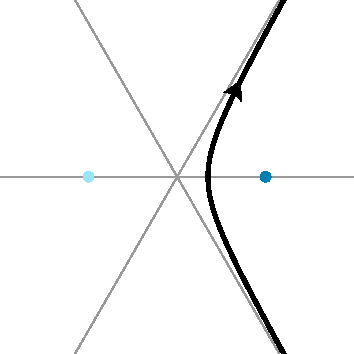
\includegraphics{figures/u_contour_3.pdf} \\[1em]
{\small The contour $\Gamma$ in the $u$ plane.}
\end{center}
With the substitution $t = 2uy^{1/2}$, we can rewrite the Airy integral as
\[ \Ai(y) = y^{1/2}\;\frac{i}{\pi} \int_{y^{-1/2} \Gamma} \exp\left[-\tfrac{2}{3}y^{3/2} \left(4u^3 - 3u\right)\right]\,du. \]
We've rescaled the contour by a factor of two, but it still approaches $\infty$ in the desired way. Note that $4u^3 - 3u$ is the third Chebyshev polynomial.
\begin{itemize}
\item By considering other Chebyshev polynomials, we can situate the Airy function within the family of {\em Airy-Lucas functions}.
\item The arguments we'll do for the Airy function work essentially the same for all Airy-Lucas functions, so we'll go straight to the general case.
\item However, since the Airy function is a classic example in the study of Borel summation and resurgence, it may be useful to see on its own. Appendix~\textbf{[airy-appendix]} shows the same arguments in this special case.
\end{itemize}


\subsection{Airy--Lucas}
The Airy-Lucas equation is
\begin{equation}\label{eqn:airy-lucas}
\left[\big(\tfrac{\partial}{\partial y}\big)^2 - (m-1) y^{-1} \tfrac{\partial}{\partial y} - y^{n-2}\right] \psi = 0
\end{equation}
with $n \in \{3, 4, 5, \ldots\}$ and $m \in \{1, 2, \ldots, r-1\}$. A few solutions are given by the Airy-Lucas functions~\textcolor{magenta}{[Charbonnier et al., equation~3.6]}
\[ \widehat{\Ai}^{(k)}_{n, m-1}(y) = \left\{\begin{array}{ll}1 & j \text{ even} \\ i & j \text{ odd}\end{array}\right\} \frac{y^{m/2}}{\pi} \int_{\Lambda^{(j)}} \exp\left[\tfrac{2}{n} y^{n/2}\,T_n(u)\right]\,U_{m-1}(u)\,du, \]
where $\Lambda^{(k)}$ is the Lefschetz thimble through $u = \cos\big(\tfrac{k}{n}\pi\big)$.
\subsubsection{Rewriting as a \textcolor{DarkCyan}{modified Bessel (?)} equation}
We can distill the most interesting parts of the Airy-Lucas function by writing
\[ \widehat{\Ai}^{(k)}_{n, m-1}(y) = \textcolor{magenta}{\text{const.}}\,y^{\textcolor{DarkCyan}{m/2}}\,K\big(\tfrac{2}{n} y^{n/2}\big), \]
where
\begin{equation}\label{integral:mod-bessel-rational}
K(z) = \textcolor{magenta}{\text{const.}} \int_{z^{-\textcolor{DarkCyan}{1/n}}\Lambda^{(k)}} \exp\left[-z T_n(u)\right]\,U_{m-1}(u)\,du.
\end{equation}
Saying that $\widehat{\Ai}^{(k)}_{n, m-1}$ satisfies the Airy-Lucas equation is equivalent to saying that $K$ satisfies the \textcolor{DarkCyan}{modified Bessel (?)} equation
\begin{equation}%%\label{eqn:mod-bessel}
\left[z^2 \big(\tfrac{\partial}{\partial z}\big)^2 + z \tfrac{\partial}{\partial z} - \big[\big(\textcolor{DarkCyan}{\tfrac{m}{n} (?)}\big)^2 + z^2\big]\right] \varphi = 0.
\end{equation}
In fact, as we'll see in Section~\textcolor{magenta}{?}, $K$ is the modified Bessel function $K_{\textcolor{DarkCyan}{m/n}}$.

Like we did in equation~\ref{eqn:reg-mod-bessel}, we can rewrite the modified Bessel equation above as
\begin{equation}%%\label{eqn:reg-mod-bessel}
\left[ \big[ \big(\tfrac{\partial}{\partial z}\big)^2 - 1 \big] + z^{-1} \tfrac{\partial}{\partial z} - \big(\textcolor{DarkCyan}{\tfrac{m}{n}}\big)^2 z^{-2} \right] \varphi = 0.
\end{equation}

\textcolor{orange}{[copy the result of Bessel with parameter $\nu=m/n$.]}

\subsection{Modified Bessel}

\textcolor{magenta}{[For this, we lift to a countable cover; see {\tt airy-resurgence.tex}, currently \S 6.4]}

\subsection{Higher Airy}

The higher Airy equation is
\begin{equation}\label{eqn:airy-lucas}
\left[\big({-}\tfrac{\partial}{\partial y}\big)^{n-1} - y\right] \psi = 0
\end{equation}
with $n \in \{3, 4, 5, \ldots\}$. A few solutions are given by the hyper-Airy functions~\textcolor{magenta}{[Charbonnier et al., equation~3.6]}

\color{Peru}
With
\begin{align*}
z & = (-1)^{n-1} \tfrac{n-1}{n} y^{n/(n-1)} & w & = (-1)^n (n-1) y^{1/(n-1)} u,
\end{align*}
we have
\begin{align*}
\widetilde{\Ai}^{(k)}_n(y) & = \frac{\exp\big(\pi ik \tfrac{n-2}{n-1}\big)}{2\pi i} \int_{\Lambda^{(j)}} \exp\left[\tfrac{1}{n}w^n - yw\right]\,dw \\
& = \frac{\exp\big(\pi ik \tfrac{n-2}{n-1}\big)}{2\pi i} \int_{\Lambda^{(j)}} \exp\left[\tfrac{1}{n}w \left(w^{n-1} - ny\right)\right]\,dw \\
& = \frac{\exp\big(\pi ik \tfrac{n-2}{n-1}\big)}{2\pi i} \int_{\Lambda^{(j)}} \exp\left[\tfrac{1}{n}w \big((n-1)^{n-1} yu^{n-1} - ny\big)\right]\,dw \\
& = \frac{\exp\big(\pi ik \tfrac{n-2}{n-1}\big)}{2\pi i} \int_{\Lambda^{(j)}} \exp\left[\tfrac{1}{n}yw \big((n-1)^{n-1} u^{n-1} - n\big)\right]\,dw \\
& = \frac{\exp\big(\pi ik \tfrac{n-2}{n-1}\big)}{2\pi i} \int_{\Lambda^{(j)}} \exp\left[(-1)^n \tfrac{n-1}{n} y^{n/(n-1)} u\big((n-1)^{n-1} u^{n-1} - n\big)\right]\,dw \\
& = \frac{\exp\big(\pi ik \tfrac{n-2}{n-1}\big)}{2\pi i} \int_{\Lambda^{(j)}} \exp\left[-z\big((n-1)^{n-1} u^n - nu\big)\right]\,dw \\
& = (-1)^n (n-1) \frac{\exp\big(\pi ik \tfrac{n-2}{n-1}\big)}{2\pi i} y^{1/(n-1)}\int_{\Lambda^{(j)}} \exp\left[-z\big((n-1)^{n-1} u^n - nu\big)\right]\,du \\
& = (-1)^n (n-1) \frac{\exp\left(\pi ik \big(1 - \tfrac{1}{n-1}\big)\right)}{2\pi i} y^{1/(n-1)}\int_{\Lambda^{(j)}} \exp\left[-z\big((n-1)^{n-1} u^n - nu\big)\right]\,du \\
& = (-1)^{n+k} (n-1) \frac{\exp\big({-}\pi i \tfrac{k}{n-1}\big)}{2\pi i} y^{1/(n-1)}\int_{\Lambda^{(j)}} \exp\left[-z\big((n-1)^{n-1} u^n - nu\big)\right]\,du \\
\end{align*}
\color{black}
\[ \widetilde{\Ai}^{(k)}_n(y) = (-1)^{n+k} (n-1) \frac{\exp\big({-}\pi i \tfrac{k}{n-1}\big)}{2\pi i} y^{1/(n-1)}\int_{\Lambda^{(j)}} \exp\left[-z\big((n-1)^{n-1} u^n - nu\big)\right]\,du \\, \]
where $\Lambda^{(k)}$ is the Lefschetz thimble through $u = \cos\big(\tfrac{k}{n}\pi\big)$.
\subsubsection{Rewriting as a \textcolor{magenta}{(???)} equation}
We can distill the most interesting parts of the hyper-Airy function by writing
\[ \widetilde{\Ai}^{(k)}_n(y) = \textcolor{magenta}{\text{const.}}\,y^{1/(n-1)}\,K\left((-1)^n\,\tfrac{n-1}{n}\,y^{n/(n-1)}\right), \]
where
\begin{equation}
K(z) = \textcolor{magenta}{\text{const.}} \int_{\textcolor{magenta}{\text{const.}(n)} z^{-\textcolor{DarkCyan}{1/n}}\Lambda^{(k)}} \exp\left[-z\big((n-1)^{n-1} u^n - nu\big)\right]\,du.
\end{equation}
Saying that $\widetilde{\Ai}^{(k)}_n$ satisfies the higher Airy equation is equivalent to saying that $K$ satisfies an equation of the form
\begin{equation}\label{eqn:higher-Airy}
\left[ \big[ \big({-}\tfrac{\partial}{\partial z}\big)^{n-1} - 1 \big] - c_n^{(1)} z^{-1} \big({-}\tfrac{\partial}{\partial z}\big)^{n-2} - c_n^{(2)} z^{-2} \big({-}\tfrac{\partial}{\partial z}\big)^{n-3} - \ldots - c_n^{(n-1)} z^{-(n-1)} \right] \varphi = 0.
\end{equation}
The sub-leading coefficients are the triangular numbers
\[ c_n^{(1)} = \frac{n(n-1)}{2}. \]
\color{DarkCyan}
The later coefficients can be written as\footnote{Many thanks to Peter Taylor for noticing this [\url{https://mathoverflow.net/q/422337/1096}].}
\[ c_n^{(k)} = \frac{b_n^{(k)}}{n^k}\,(n+1)^{\underline{k+2}} \]
in terms of the polynomials

\begin{align*}
b_n^{(2)} & = & \tfrac{1}{24} \\
b_n^{(3)} & = & \tfrac{1}{48} n \\
b_n^{(4)} & = & \tfrac{73}{5760} n^2 & + & \tfrac{1}{1152} n & - & \tfrac{1}{2880} \\
b_n^{(5)} & = & \tfrac{11}{1280} n^{3} & + & \tfrac{1}{768} n^{2} & - & \tfrac{1}{1920} n \\
b_n^{(6)} & = & \tfrac{3625}{580608} n^{4} & + & \tfrac{61}{41472} n^{3} & - & \tfrac{181}{322560} n^{2} & - & \tfrac{1}{41472} n & + & \tfrac{1}{181440}. 
\end{align*}


Searching for 580608 in the OEIS turns up the leading coefficients $\beta^{(k)}$ of these polynomials, which are listed as {\tt A249276} and {\tt A249277}. They're defined by the identity [Yang, ``Approximations for Constant $e$ and Their Applications'']
\[ \frac{1}{e} \left(\frac{n}{n-1}\right)^{n-1} = 1 - \frac{1/2}{n} - \frac{\beta^{(2)}}{n^2} - \frac{\beta^{(3)}}{n^3} - \frac{\beta^{(4)}}{n^4} - \frac{\beta^{(5)}}{n^5} - \ldots, \]
which tells us that
\[ \frac{1}{e} \left(\frac{n}{n-1}\right)^{n-1} = 1 - \frac{1/2}{n} - \frac{b_n^{(2)}}{n^2} - \frac{b_n^{(3)}}{n^4} - \left[\frac{b_n^{(4)}}{n^6} + o\left(\frac{1}{n^5}\right)\right] - \left[\frac{b_n^{(5)}}{n^8} + o\left(\frac{1}{n^6}\right)\right] - \ldots. \]
The last coefficient can be written as
\[ c_n^{(n-1)} = \left(\frac{n-1}{n}\right)^{n-1} \left(\frac{1}{n-1}\right)^{\underline{n-1}}, \]
giving
\[ b_n^{(n-1)} = (n-1)^{n-1} \left(\frac{1}{n-1}\right)^{\underline{n-1}} \Big/ (n+1)^{\underline{n+1}}. \]
\color{black}

\subsubsection{Higher Airy of degree $3$}
Setting $n=4$, equation \ref{eqn:higher-Airy} turns into 

\begin{equation}\label{eqn:reg-higher3}
\left[\frac{\partial^3}{\partial z^3}+1+\frac{6}{z}\frac{\partial^2}{\partial z^2}-\frac{35}{8}\frac{1}{z^2}\frac{\partial}{\partial z}+\frac{315}{16}\frac{1}{z^3}\right]\varphi=0
\end{equation}

We're going to look for functions $v_\alpha$ whose Laplace transforms $\laplace_{\zeta, \alpha} v_\alpha$ satisfy equation~\ref{eqn:reg-higher3}. We'll succeed when $\alpha^3 + 1 = 0$.%, and we'll see that $K$ is a scalar multiple of $\laplace_{\zeta, 1} v_1$.

We can see from Section~\ref{L-int-op} that $\laplace_{\zeta, \alpha} v$ satisfies the differential equation~\ref{eqn:reg-higher3} if and only if $v$ satisfies the integral equation
\begin{equation}\label{int-eq:higher3}
\left[ \big[ \zeta^2 - 1 \big] - \fracderiv{-1}{\zeta}{\alpha} \circ \zeta - \big(\tfrac{1}{3}\big)^2 \fracderiv{-2}{\zeta}{\alpha} \right] v = 0.
\end{equation}
It's tempting to differentiate both sides of this equation until we get
\begin{equation}\label{diff-eq:higher3}
\left[ \big(\tfrac{\partial}{\partial \zeta}\big)^2 \circ \big[ \zeta^2 - 1 \big] - \tfrac{\partial}{\partial \zeta} \circ \zeta - \big(\tfrac{1}{3}\big)^2 \right] v = 0,
\end{equation}
which is easier to solve. Unfortunately, a solution of equation~\ref{diff-eq:spatial-mod-bessel} won't satisfy equation~\ref{int-eq:spatial-mod-bessel} in general. However, as we learned in Section~\ref{shifting}, a solution of equation~\ref{diff-eq:spatial-mod-bessel} {\em will} satisfy equation~\ref{int-eq:spatial-mod-bessel} if it's slight and locally integrable at $\zeta = \alpha$.

This is great news, because equation~\ref{diff-eq:spatial-mod-bessel} has a regular singularity at each root of $\zeta^2 - 1$, and the Frobenius method often gives a slight solution at each regular singular point. We can see the regular singularities by moving the derivatives to the right:
\[ \left[ (\zeta^2 - 1) \big(\tfrac{\partial}{\partial \zeta}\big)^2 + 3\zeta \tfrac{\partial}{\partial \zeta} + \big[ 1 - \big(\tfrac{1}{3}\big)^2 \big] \right] v = 0. \]

In Sections \ref{pos-root}\,--\,\ref{neg-root}, we'll see this approach succeed. For each root $\alpha$, we'll find a solution $v_\alpha$ of equation~\ref{diff-eq:spatial-mod-bessel} which is slight and locally integrable at $\zeta = \alpha$. We know the function $\laplace_{\zeta, \alpha} v_\alpha$ will satisfy equation~\ref{eqn:reg-mod-bessel}, and we can even find its asymptotics from the order $\tau_\alpha$ of $v_\alpha$. We learned in Section~\ref{translation} that
\[ \laplace_{\zeta, \alpha} v_\alpha = e^{-\alpha z} V_\alpha \]
where $V_\alpha = \laplace_{\zeta_\alpha, 0} v_\alpha$ and $\zeta = \alpha + \zeta_\alpha$. We can see from Section~\ref{reg-decay} that $V_\alpha\in z^{-\tau_\alpha}\C[\![z^{-1}]\!]$, so we further decompose
\[ \laplace_{\zeta, \alpha} v_\alpha = e^{-\alpha z} z^{-\tau_\alpha} W_\alpha, \]
with $W_\alpha\in\C[\![z^{-1}]\!]$.
\color{Peru}
\begin{align*}
\left[ \big(\tfrac{\partial}{\partial \zeta}\big)^2 \circ (\zeta - 1)(\zeta + 1) - \tfrac{\partial}{\partial \zeta} \circ \zeta - \big(\tfrac{1}{3}\big)^2 \right] v & = 0
\end{align*}
\color{Sienna}
\begin{align*}
\left[ \big[ 2 + 2(2\zeta) \tfrac{\partial}{\partial \zeta} + (\zeta^2 - 1) \big(\tfrac{\partial}{\partial \zeta}\big)^2 \big] - \big[ 1 + \zeta \tfrac{\partial}{\partial \zeta} \big] - \big(\tfrac{1}{3}\big)^2 \right] v & = 0 \\
\left[ (\zeta^2 - 1) \big(\tfrac{\partial}{\partial \zeta}\big)^2 + 3\zeta \tfrac{\partial}{\partial \zeta} + \big[ 1 - \big(\tfrac{1}{3}\big)^2 \big] \right] v & = 0 \\
\left[ (\zeta - 1)(\zeta + 1) \big(\tfrac{\partial}{\partial \zeta}\big)^2 + 3\zeta \tfrac{\partial}{\partial \zeta} + \big[ 1 - \big(\tfrac{1}{3}\big)^2 \big] \right] v & = 0
\end{align*}
\color{black}
%%In terms of the coordinate $\zeta_\alpha$ with $\zeta = \alpha + \zeta_\alpha$, this equation is written
%%\begin{equation}\label{eqn:centered-mod-bessel}
%%\[ \left[ \big[ \zeta_\alpha (\zeta_\alpha + 2\alpha) + \alpha^2 - 1 \big] + \fracderiv{-1}{\zeta_\alpha}{0} \circ \big[ \zeta_\alpha + \alpha \big] - \big(\tfrac{1}{3}\big)^2 \fracderiv{-2}{\zeta_\alpha}{0} \right] w = 0. \]
%%\end{equation}
\subsubsection{Focus on $\zeta = 1$}\label{pos-root}
Let's find a solution of equation~\ref{diff-eq:spatial-mod-bessel} which is slight and locally integrable at $\zeta = 1$. Define a new coordinate $\zeta_1$ on $\C$ so that $\zeta = 1 + \zeta_1$. In this coordinate, equation~\ref{diff-eq:spatial-mod-bessel} looks like
\begin{equation}%%\label{diff-eq:spatial-mod-bessel-pos}
\left[\zeta_1(2 + \zeta_1) \big(\tfrac{\partial}{\partial \zeta_1}\big)^2 + 3(1 + \zeta_1) \tfrac{\partial}{\partial \zeta_1} + \big[1 - \big(\tfrac{1}{3}\big)^2\big]\right] v = 0.
\end{equation}
With another change of coordinate, given by $\zeta_1 = -2\xi_1$, we can rewrite equation~\ref{diff-eq:spatial-mod-bessel} as the hypergeometric equation
\begin{equation}\label{diff-eq:hypergeom-pos}
\left[\xi_1 (1 - \xi_1) \big(\tfrac{\partial}{\partial \xi_1}\big)^2 + 3(\tfrac{1}{2} - \xi_1) \tfrac{\partial}{\partial \xi_1} - \big[1 - \big(\tfrac{1}{3}\big)^2\big]\right] v = 0.
\end{equation}
Looking through the twenty-four expressions for Kummer's six solutions, we find one \cite[formula~15.10.12]{dlmf} which is manifestly slight and locally integrable at $\xi_1 = 0$:
\begin{alignat*}{2}
v_1 &=\;& \hphantom{-i\sqrt{2}}\,\xi_1^{-1/2} & F\big(\tfrac{1}{6}, \tfrac{5}{6}; \tfrac{1}{2}; \xi_1\big) \\
&=\;& -i\sqrt{2}\,\zeta_1^{-1/2} & F\big(\tfrac{1}{6}, \tfrac{5}{6}; \tfrac{1}{2}; -\tfrac{1}{2}\zeta_1\big)
\end{alignat*}
From the argument in Section~\ref{big-idea}, we know that $\laplace_{\zeta, 1} v_1$ satisfies equation~\ref{eqn:mod-bessel}, and can be written as $e^{-z} V_1$, where $V_1 = \laplace_{\zeta_1, 0} v_1$. Since $v_1$ has order $-1/2$, the decomposition $V_1 = z^{1/2} W_1$ makes $W_1$ asymptotic to a scalar multiple of $z^{-1}$ at $z = \infty$.
\subsubsection{Focus on $\zeta = -1$}\label{neg-root}
Let's find a solution of equation~\ref{diff-eq:spatial-mod-bessel} which is slight and locally integrable at $\zeta = -1$. In the rescaled coordinate from Section~\ref{pos-root}, this is the point $\xi_1 = 1$. Looking again through Kummer's table of solutions, we find another expression \cite[formula~15.10.14]{dlmf} which is manifestly slight and locally integrable at $\xi_1 = 1$:
\begin{alignat*}{2}
v_{-1} &=\;& (1-\xi_1)^{-1/2} & F\big(\tfrac{1}{6}, \tfrac{5}{6}; \tfrac{1}{2}; 1-\xi_1\big) \\
&=\;& \sqrt{2}\,\zeta_{-1}^{-1/2} & F\big(\tfrac{1}{6}, \tfrac{5}{6}; \tfrac{1}{2}; \tfrac{1}{2}\zeta_{-1}\big)
\end{alignat*}
where $\zeta_{-1}$ is the coordinate with $\zeta = -1 + \zeta_{-1}$. From the argument in Section~\ref{big-idea}, we know that $\laplace_{\zeta, -1} v_{-1}$ satisfies equation~\ref{eqn:mod-bessel}, and can be written as $e^z V_{-1}$, where $V_{-1} = \laplace_{\zeta_{-1}, 0} v_{-1}$. Since $v_{-1}$, like our other solution, has order $-1/2$, the same decomposition $V_{-1} = z^{1/2} W_{-1}$ makes $W_{-1}$ asymptotic to a scalar multiple of $z^{-1}$ at $z = \infty$.

In this example, $v_1$ and $v_{-1}$ happen to be related by a symmetry: the M\"{o}bius transformation that pulls $\zeta$ back to $-\zeta$. Kummer's solutions typically come from six different hypergeometric equations, which are related by the M\"{o}bius transformations that permute their singularities. In our case, though, exchanging $1$ with $-1$ keeps equation~\ref{diff-eq:spatial-mod-bessel} the same.

\color{DodgerBlue}
If we'd followed the routine from Section~\ref{pos-root}, rewriting equation~\ref{diff-eq:spatial-mod-bessel} in the coordinate $\zeta_{-1}$ and then rewriting it again in a more recognizable form, we would've arrived at the hypergeometric equation
\[ \left[\xi_{-1} (1 - \xi_{-1}) \big(\tfrac{\partial}{\partial \xi_{-1}}\big)^2 + 3(\tfrac{1}{2} - \xi_{-1}) \tfrac{\partial}{\partial \xi_{-1}} - \big[1 - \big(\tfrac{1}{3}\big)^2\big]\right] v = 0, \]
where $\zeta_{-1} = 2\xi_{-1}$. This is the same as what we'd get by substituting $\xi_{-1}$ for $\xi_1$ in Section~\ref{pos-root}! In other words, the holomorphic map that pulls $\xi_{-1}$ back to $\xi_1$.

\color{black}

\subsection{Generalized Airy}

\section{Third-order exponential integrals}
\begin{itemize}
\item Reduce to
\[ I(z) = \int \exp\left[-z\big(u^3 + pu + q)\right]\,du \]
using change of coordinate.
\item When $p \neq 0$, can reduce further to
\[ I(z) = p^{1/2} e^{-qz} K_{1/3}(p^{3/2} z). \]
\item As $p$ goes to zero, $I(z)$ degenerates to
\[ \left(\tfrac{1}{2}\right)^{2/3} e^{-qz} \Gamma(\tfrac{1}{3}) z^{-1/3} = \left(\tfrac{1}{2}\right)^{2/3} e^{-qz} \laplace_{\zeta,0}(\zeta^{-2/3}) = \left(\tfrac{1}{2}\right)^{2/3} \laplace_{\zeta_{-q},q}(\zeta^{-2/3}). \]
\end{itemize}


\color{orange}
\section*{Outline}

\textbf{Title: Borel regularity and Resurgence of Exponential Integrals}

\begin{enumerate}
\item introduction
\begin{itemize}
\item Exponential integrals
\begin{itemize}
\item they are function of $z$ and they are defined from the data of $(X,f)$ and $[\mathcal{C}], [\nu]$
\item the choice of the path $\mathcal{C}$: 
\begin{itemize}
\item $\mathcal{C}\in H^{B,z}_{n}(X,f)$
\item Witten's formalism, $\mathcal{C}$ is a Lefschetz thimbles (or steepest descendent path)
\end{itemize}
\item they define a paring between the relative homology (rapid decaying homology)$H^{B,z}_{\bullet}(X,f)$ and the twisted de Rham cohomology  $H_{dR,z}^{\bullet}(X,f)$
\begin{itemize}
\item there is a comparison isomorphism (Maxim)
\end{itemize}
\item varying $z$ we have the Stokes phenomena
\item as $z\to\infty$, the asymptotic expansion of $I$ is a divergent series $\tilde{I}$, usually of Gevrey-class
\begin{itemize}
\item {\it exact resurgence relation} (Berry--Howls): divergence encodes contributions from other critical values
\item it is an example of resurgent series (\'Ecalle)
\item $\tilde{I}$ is resurgent in $\C\setminus\lbrace \text{poles of } \nu\,, \text{cirtical values of } f\rbrace$
\item it is a toy example of resurgent series because there are only finitely many singularities in the Borel plane
\item we have to compute the \textbf{Stokes constants} relative to the singular points in $B$ to fully understand $B$. There are two methods to compute Stokes constants: $\bullet$ geometric: using intersection theory of thimbles (Picard--Lefschtez, Witten, Maxim), $\bullet$ analytic: using \'Ecalle formalism   
\end{itemize} 
\end{itemize}
\item what are exponential integrals? \textcolor{gray}{has to be done}
\begin{itemize}
\item motivation
\begin{itemize}
\item In the classical theory of special functions, exponential integrals are often used to express solutions of linear differential and difference equations.
\item In physics ??
\item Geometrically they represent a Poincar\'e pairing (as explained by Kontsevich in \textbf{IHES lectures}).
\end{itemize}
\end{itemize}
\item What is the class of ODEs that we study? \textcolor{gray}{has to be done}
\item State results about resurgence of exponential integrals and Stokes phenomena
\begin{itemize}
\item Thimbles integrals [Kontsevich]: geometric computation of Stokes constants \textcolor{gray}{has to be done}
\item ODE and fractional derivative formula [{\tt draft2}]
\item if hypergeometric functions appear in a large class of examples: integral formulas for hypergeometric functions \textcolor{gray}{has to be done}
\end{itemize}
\end{itemize}
\item Formalism for Laplace transform [{\tt draft2}, ``The geometry of the Laplace transform'']
\begin{enumerate}
\item Analytic
\begin{enumerate}
\item Introduction
\item Brief revew of translation surfaces (we can refer to this from the introduction if we need to)
\item The Laplace transform of a holomorphic function
\begin{enumerate}
\item Over an ordinary point
\item Over a branch point
\item Differential equation
\end{enumerate}
\item Relating differential equations in the frequency domain to integral equations in the position domain
\end{enumerate}
\item Formal
\begin{enumerate}
\item Laplace transform of a formal series
\item Borel transform
\item Relating differential equations in the frequency variable to integral equations in the position variable
\end{enumerate}
\end{enumerate}
\item Review of integral equations
\begin{itemize}
\item Existence of solutions
\item Fractional integrals and derivatives
\item Going between integral and differential equations (slight functions)
\end{itemize}
\item General cases
\begin{enumerate}
\item Borel regularity
\begin{itemize}
\item General ODE of the form
\[ \left[ P\big(\tfrac{\partial}{\partial z}\big) + z^{-1} Q\big(\tfrac{\partial}{\partial z}\big) + z^{-2} R(z^{-1}) \right] \Phi = 0, \]
where $P$ is a polynomial, $Q$ is a polynomial of one degree lower, and $R$ is an entire function~\text[see {\tt airy-resurgence} and written notes]
\begin{itemize}
\color{DarkCyan}
\item More generally, for $P$ of degree $n$, we should be able to handle
\[ \left[ P\big(\tfrac{\partial}{\partial z}\big) + z^{-1} Q_1\big(\tfrac{\partial}{\partial z}\big) + z^{-2} Q_2\big(\tfrac{\partial}{\partial z}\big) + \ldots + z^{-(n-1)} Q_{n-1}\big(\tfrac{\partial}{\partial z}\big) + z^{-n} R(z^{-1}) \right] \Phi = 0, \]
where $Q_k$ has degree $n-k$. \textcolor{gray}{has to be done}
\begin{itemize}
\item We want the most general ODE with a regular singularity at $z = 0$ and its only other singularity, typically irregular, at $z = \infty$. \textcolor{gray}{has to be done}
\item The singularity at $\infty$ should only be regular for an Euler equation. \textcolor{gray}{has to be done}
\end{itemize}
\color{orange}
\item Show that we can find a slight solution at each critical value.
\item Show that $\hat{\iota} = \tilde{\iota}$, where:
\begin{itemize}
\item $I = \laplace \iota$
\item $\hat{\iota}$ is the Taylor expansion of $\iota$
\item $\tilde{I}$ is the asymptotic series of $I$
\item $\tilde{\iota} = \borel \tilde{I}$
\item Idea: Show that $\hat{\iota}$ and $\tilde{\iota}$ have matching asymptotics at $\zeta = 0$. Since they both satisfy the position-domain integral equation, they must coincide.
\end{itemize}
\end{itemize}
\item General thimble integral (conditions?)
\begin{itemize}
\item Proof of Borel regularity
\item $3/2$-derivative formula
\item Contour argument
\end{itemize}
\end{itemize}
\item Resurgence
\begin{itemize}
\item Explain how Borel regularity relates resurgence of formal series to resurgence of holomorphic functions in the position domain. \textcolor{gray}{think more about what we're trying to say here}
\item Relate to Ecalle's formalism and the alien derivative
\item Stokes factors
\begin{itemize}
\item For ODEs
\item For thimble integrals
\end{itemize}
\end{itemize}
\end{enumerate}
\item Examples \textcolor{gray}{make sure each example contains a computation of the Borel transform, so we can see it matches}
\begin{enumerate}
\item The Airy example
\begin{itemize}
\item $I(z)$ is a solution of a linear ODE. We explicitly find its Borel transform, knowing the nature of singularities and the asymptotic behaviour of a basis of solution for the ODE  [{\tt airy-resurgence}]
\item Compute Stokes constants
\begin{itemize}
\item Using fractional derivative formula and Borel transform computation [{\tt draft2}]
\item Using Picard-Lefschetz theory (Pham, Kontsevich, etc.)
\end{itemize}
\item Comparison with the literature \textcolor{gray}{has to be done}
\begin{itemize}
\item Mari\~{n}o
\item Sauzin
\item Kontsevich slides
\item Kawai--Takei? [might take too long to understand well enough]
\end{itemize}
\end{itemize}
\item The Airy--Lucas examples
\begin{itemize}
\item Compute Borel transform [{\tt airy-resurgence}]
\item Compute Stokes constants \textcolor{gray}{has to be done}
\end{itemize}
\item Bessel 0 (it is different because we have infinite cover)
\begin{itemize}
\item Compute Stokes constants [{\tt draft2}]
\end{itemize}
\item Bessel $\mu$ (follows from Bessel 0)
\begin{itemize}
\item Compute Stokes constants [{\tt modified Bessel}]
\end{itemize}
\item The generalized Airy example
\item The vibrating beam example
\begin{itemize}
\item In addition to the simple example, maybe we can do an example where the equation on the spatial domain includes fractional integrals, since Andy is interested in that sort of thing
\end{itemize}
\end{enumerate}
\end{enumerate}

\color{black}

\appendix

\section{Integro-differential equations}
\subsection{Existence of solutions}
\subsubsection{Algebraic integral operators}
Take a simply connected open set $\Omega \subset \C$ that touches but doesn't contain $\zeta = 0$. Let $\holoL{\infty}(\Omega)$ be the space of bounded holomorphic functions on $\Omega$ with the supremum norm $\|\cdot\|_\infty$. For any $\sigma \in \R$, multiplying by $\zeta^{-\sigma}$ maps $\holoL{\infty}(\Omega)$ isomorphically onto another space of holomorphic functions on $\Omega$. We'll call this space $\holoL{\infty, \sigma}(\Omega)$ and give it the norm $\|f\|_{\infty, \sigma} = \|\zeta^\sigma f\|_\infty$, so that
\begin{align*}
\holoL{\infty}(\Omega) & \to \holoL{\infty, \sigma}(\Omega) \\
\phi & \mapsto \zeta^{-\sigma} \phi
\end{align*}
is an isometry. More generally,
\begin{align*}
\holoL{\infty, \rho}(\Omega) & \to \holoL{\infty, \rho+\delta}(\Omega) \\
f & \mapsto \zeta^{-\delta} f
\end{align*}
is an isometry for all $\rho \in \R$ and $\delta \in [0, \infty)$. This reduces to the previous statement when $\rho = 0$. For each $\delta \in [0, \infty)$, the functions in $\holoL{\infty, \rho}(\Omega)$ belong to $\holoL{\infty, \rho+\delta}(\Omega)$ too, and the inclusion map $\holoL{\infty, \rho}(\Omega) \hookrightarrow \holoL{\infty, \rho+\delta}(\Omega)$ has norm $\|\zeta^\delta\|_\infty$. Conceptually, $\|\zeta^\delta\|_\infty$ measures of the size of $\Omega$, so let's write it as $M^\delta$ with $M = \|\zeta\|_\infty$.

Since $\holoL{\infty}(\Omega)$ is a Banach algebra, the function space $\holoL{\infty, \infty}(\Omega) := \bigcup_{\sigma \in \R} \holoL{\infty, \sigma}(\Omega)$ is a graded algebra, with a different norm on each grade. For each $\rho, \delta \in \R$, multiplication by a function $m \in \holoL{\infty, \delta}(\Omega)$ gives a map $\holoL{\infty, \rho}(\Omega) \to \holoL{\infty, \rho+\delta}(\Omega)$ with norm $\|m\|_{\infty, \delta}$.

We'll study integral operators $\mathcal{G} \maps \holoL{\infty, \rho}(\Omega) \to \holoL{\infty, \sigma}(\Omega)$ of the form
\[ [\mathcal{G}f](a) = \int_{\zeta = 0}^{a} g(a, \cdot)\,f\,d\zeta, \]
where the kernel $g$ is an algebraic function over $\C^2$ which can be singular on $\Delta$, the diagonal.\footnote{Thanks to Alex Takeda for suggesting this.} To avoid ambiguity, we fix a branch of $g$ to use at the start of the integration path. The domain of $g$ is a covering of $\C^2$ which can be branched over $\Delta$. Continuing $g$ around $\Delta$ changes its phase by a root of unity, leaving its absolute value the same \textbf{[check]}. That makes $|g|$ a well-defined function on $\C^2 \smallsetminus \Delta$, which we can use to bound $\|\mathcal{G}\|$.

For each $a \in \C$, the expression $|g(a, \cdot)\,d\zeta|$ defines a {\em density} on $\Omega \smallsetminus \{a\}$---a norm on the tangent bundle which is compatible with the conformal structure. The square of a density is a Riemannian metric. Let $\ell^{\sigma, \rho}_{g, \Omega}(a)$ be the distance from $\zeta = 0$ to $a$ with respect to the density $|\zeta(a)^\sigma\,g(a, \cdot)\,\zeta^{-\rho}\,d\zeta|$ on $\Omega \smallsetminus \{a\}$. The bound
\begin{align*}
\big|[\zeta^\sigma \mathcal{G}f](a)\big| & \le \left| \zeta(a)^\sigma \int_{\zeta = 0}^{a} g(a, \cdot)\,f\,d\zeta \right| \\
& \le \int_{\zeta = 0}^{a} |\zeta^\sigma f|\,|\zeta(a)^\sigma\,g(a, \cdot)\,\zeta^{-\rho}\,d\zeta| \\
& \le \|f\|_{\infty, \sigma} \int_{\zeta = 0}^{a} |\zeta(a)^\sigma\,g(a, \cdot)\,\zeta^{-\rho}\,d\zeta|
\end{align*}
holds for any integration path. Taking the infimum over all paths, we see that
\[ \big|[\mathcal{G}f](a)\big| \le \ell^{\sigma, \rho}_{g, \Omega}(a)\,\|f\|_\infty. \]
so $\|\mathcal{G}\| \le \sup_{a \in \Omega} \ell^{\sigma, \rho}_{g, \Omega}(a)$. Crucially, we can always make $\|\mathcal{G}\|$ a contraction by restricting $\Omega$.
\subsubsection{The example of fractional integrals}
Setting $g(a, a') = (\zeta(a) - \zeta(a'))^{-\lambda-1}$ with $\lambda \in (-\infty, 0)$, we get the fractional integral $\partial^\lambda_{\zeta \text{ from } 0}$. The shortest path from $\zeta = 0$ to $a$ with respect to $|\zeta(a)^{\rho+\lambda}\,g(a, \cdot)\,\zeta^{-\rho}\,d\zeta|$ is the same as the shortest path with respect to $|d\zeta|$ \textcolor{magenta}{[check]}. It follows that
\begin{align*}
\ell^{\sigma, \rho}_{g, \Omega}(a) & = \int_0^{|\zeta(a)|} |\zeta(a)|^{\rho+\lambda}\,(|\zeta(a)| - r)^{-\lambda-1}\,r^{-\rho}\,dr \\
& = |\zeta(a)|^{\rho+\lambda} \int_0^1 \,(|\zeta(a)| - |\zeta(a)| t)^{-\lambda-1}\,(|\zeta(a)| t)^{-\rho}\,|\zeta(a)|\,dt \\
& = |\zeta(a)|^{\rho+\lambda-\lambda-1-\rho+1} \int_0^1 \,(1-t)^{-\lambda-1}\,t^{-\rho}\,dt \\
& = \int_0^1 \,(1-t)^{-\lambda-1}\,t^{-\rho}\,dt \\
& = B(-\lambda,\,1-\rho).
\end{align*}
The beta function $B$ can be written more explicitly as
\[ B(-\lambda,\,1-\rho) = \frac{\Gamma(-\lambda)\,\Gamma(1-\rho)}{\Gamma(1-\lambda-\rho)}. \]
Now we can see that for each $\lambda \in (-\infty, 0)$ and $\rho \in \R$, the fractional integral $\partial^\lambda_{\zeta \text{ from } 0}$ maps $\holoL{\infty, \rho}(\Omega)$ into $\holoL{\infty, \rho+\lambda}(\Omega)$, with norm $\|\partial^\lambda_{\zeta \text{ from } 0}\| \le B(-\lambda,\,1-\rho)$.
\subsubsection{Fractional integral equations near a regular singular point}\label{frac_int_exist}
\textcolor{SeaGreen}{\textbf{Angeliki:} Maybe Kato--Rellich perturbation theory can give existence immediately. It might not give uniqueness, though.}

Consider an integral operator $\mathcal{J}$ of the form
\[ p + \partial^{-1}_{\zeta \text{ from } 0} \circ q + \sum_{\lambda \in \Lambda} \partial^\lambda_{\zeta \text{ from } 0} \circ r_\lambda, \]
where:
\begin{itemize}
\item $p$ is a function in $\holoL{\infty, -1}(\Omega)$ that extends holomorphically over $\zeta = 0$, and its derivative at $\zeta = 0$ is non-zero.
\item $q$ is a function in $\holoL{\infty}(\Omega)$ that extends holomorphically over $\zeta = 0$.
\item $r_\lambda$ are functions in $\holoL{\infty}(\Omega)$.
\item $\Lambda$ is a countable subset of $(-\infty, -1)$ whose supremum is less than $-1$.
\end{itemize}
Our demand that $p$ and $q$ have convergent power series at $\zeta = 0$ can probably be relaxed; having convergent Novikov series, for example, should be enough. We could also probably replace $\partial^{-1}_{\zeta \text{ from } 0}$ with $\partial^{-1+\delta}_{\zeta \text{ from } 0} \circ \zeta^\delta$ for some $\delta \in [0, 1)$, or adjust the $\partial^\lambda_{\zeta \text{ from } 0}$ similarly.

We want to solve the equation $\mathcal{J}f = 0$. Let's look for a solution of the form $f = \zeta^{\tau-1} + \tilde{f}$ with $\tau \in (0, \infty)$ and $\tilde{f} \in \holoL{\infty, 1-\tau-\epsilon}(\Omega)$ for some $\epsilon \in (0, 1]$. When $\epsilon$ is small enough that $\Lambda \subset (-\infty, -1 - \epsilon]$, we'll see that we can always find such a solution, as long as we're willing to shrink $\Omega$. In fact, there's exactly one such solution. \textcolor{magenta}{[Add convergence conditions for $\partial^\lambda$ terms.]}

Let $p'_0$ and $q_0$ be the values of $\tfrac{\partial}{\partial \zeta} p$ and $q$, respectively, at $\zeta = 0$. We're assuming that $p$ and $q$ extend holomorphically over $\zeta = 0$, and the additional assumption that $p \in \holoL{\infty, -1}(\Omega)$ implies that $p$ has a first-order zero at $\zeta = 0$.

Since $p$ and $q$ extend holomorphically over $\zeta = 0$, and $p$ vanishes at $\zeta = 0$, we can write
\begin{alignat*}{2}
p & = p'_0 \zeta &\;+\;& \tilde{p} \\
q & = q_0 &\;+\;& \tilde{q}
\end{alignat*}
with $\tilde{p} \in \holoL{\infty, -2}(\Omega)$ and $\tilde{q} \in \holoL{\infty, -1}(\Omega)$. Then we have
\[ \mathcal{J} = p'_0\zeta + q_0\,\partial^{-1}_{\zeta \text{ from } 0} + \tilde{\mathcal{J}} \]
with
\[ \tilde{\mathcal{J}} = \tilde{p} + \partial^{-1}_{\zeta \text{ from } 0} \circ \tilde{q} + \sum_{\lambda \in \Lambda} \partial^\lambda_{\zeta \text{ from } 0} \circ r_\lambda \]
For any $\tau \in (0, \infty)$,
\[ \mathcal{J} \zeta^{\tau-1} = (p'_0 + q_0/\tau)\,\zeta^\tau + \tilde{\mathcal{J}} \zeta^{\tau-1}. \]
Setting $\tau = -q_0 / p'_0$ makes the first term vanish, leaving
\[ \mathcal{J} \zeta^{\tau-1} = \tilde{\mathcal{J}} \zeta^{\tau-1}. \]
Then the equation $\mathcal{J}f = 0$ becomes
\begin{align}
0 & = \tilde{\mathcal{J}}\zeta^{\tau-1} + \mathcal{J}\tilde{f} \nonumber \\
0 & = \tilde{\mathcal{J}}\zeta^{\tau-1} + \left[ p'_0\zeta + q_0\,\partial^{-1}_{\zeta \text{ from } 0} + \tilde{\mathcal{J}} \right]\tilde{f} \nonumber \\
-p'_0\zeta\tilde{f} & = \tilde{\mathcal{J}}\zeta^{\tau-1} + \left[ q_0\,\partial^{-1}_{\zeta \text{ from } 0} + \tilde{\mathcal{J}} \right]\tilde{f} \nonumber \\
\tilde{f} & = \left[ -\tfrac{1}{p'_0}\,\zeta^{-1} \circ \tilde{\mathcal{J}} \right]\,\zeta^{\tau-1} + \left[ \tau\,\zeta^{-1} \circ \partial^{-1}_{\zeta \text{ from } 0} - \tfrac{1}{p'_0}\,\zeta^{-1} \circ \tilde{\mathcal{J}} \right]\tilde{f}. \label{fixed-pt}
\end{align}

\color{Indigo}
\begin{center}
\begin{tikzcd}[column sep=25mm, row sep=2mm]
& & \holoL{\infty, \rho-1}(\Omega) \\
\holoL{\infty, \rho}(\Omega) \arrow[r, "\tilde{p}", "\|\tilde{p}\|_{\infty, -2}"'] & \holoL{\infty, \rho-2}(\Omega) \arrow[ru, hook, "\|\zeta\|_\infty"'] \arrow[rd, hook, "\|\zeta\|_\infty^{1-\epsilon}"'] \\
& & \holoL{\infty, \rho-1-\epsilon}(\Omega) \\
& & & \holoL{\infty, \rho-1}(\Omega) \\
\holoL{\infty, \rho}(\Omega) \arrow[r, "\tilde{q}", "\|\tilde{q}\|_{\infty, -1}"'] & \holoL{\infty, \rho-1}(\Omega) \arrow[r, "\partial^{-1}", "{B(1, 2-\rho) = \frac{1}{2-\rho}}"'] & \holoL{\infty, \rho-2}(\Omega) \arrow[ru, hook, "\|\zeta\|_\infty"'] \arrow[rd, hook, "\|\zeta\|_\infty^2"'] \\
& & & \holoL{\infty, \rho}(\Omega) \\
& & & \holoL{\infty, \rho-1}(\Omega) \\
\holoL{\infty, \rho}(\Omega) \arrow[r, "r_\lambda", "\|r_\lambda\|_\infty"'] & \holoL{\infty, \rho}(\Omega) \arrow[r, "\partial^\lambda", "{B(-\lambda, 1-\rho)}"'] & \holoL{\infty, \rho+\lambda}(\Omega) \arrow[ru, hook, "\|\zeta\|_\infty^{-1-\lambda}"'] \arrow[rd, hook, "\|\zeta\|_\infty^{-1-\epsilon-\lambda}"'] \\
& & & \holoL{\infty, \rho-1-\epsilon}(\Omega) \\
\holoL{\infty, \rho}(\Omega) \arrow[r, "\partial^{-1}", "{B(1, 1-\rho) = \frac{1}{1-\rho}}"'] & \holoL{\infty, \rho-1}(\Omega) \arrow[r, "\zeta^{-1}", "\|\zeta^{-1}\|_{\infty, 1} = 1"'] & \holoL{\infty, \rho}(\Omega) \\
\end{tikzcd}
\end{center}
\color{black}

From \textbf{[our previous discussion]}, we can work out that
\begin{align*}
\tilde{\mathcal{J}} & \maps \holoL{\infty, 1-\tau}(\Omega) \to \holoL{\infty, -\tau-\epsilon}(\Omega)\;\text{with} \\
\|\tilde{\mathcal{J}}\| & \le \left(\|\tilde{p}\|_{\infty, -2} + \tfrac{1}{1+\tau}\,\|\tilde{q}\|_{\infty, -1} \right) M^{1-\epsilon} + \sum_{\lambda \in \Lambda} B(-\lambda, \tau)\,\|r_\lambda\|_{\infty}\,M^{-1-\epsilon-\lambda}
\end{align*}
and
\begin{align*}
\tilde{\mathcal{J}} & \maps \holoL{\infty, 1-\tau-\epsilon}(\Omega) \to \holoL{\infty, -\tau-\epsilon}(\Omega)\;\text{with} \\
\|\tilde{\mathcal{J}}\| & \le \left(\|\tilde{p}\|_{\infty, -2} + \tfrac{1}{1+\tau+\epsilon}\,\|\tilde{q}\|_{\infty, -1} \right) M + \sum_{\lambda \in \Lambda} B(-\lambda, \tau+\epsilon)\,\|r_\lambda\|_{\infty}\,M^{-1-\lambda}.
\end{align*}
Since $\|\zeta^{-1}\|_{\infty, 1} = 1$, it follows that
\begin{align*}
\zeta^{-1} \circ \tilde{\mathcal{J}} & \maps \holoL{\infty, 1-\tau}(\Omega) \to \holoL{\infty, 1-\tau-\epsilon}(\Omega)\;\text{with} \\
\|\zeta^{-1} \circ \tilde{\mathcal{J}}\| & \le \left(\|\tilde{p}\|_{\infty, -2} + \tfrac{1}{1+\tau}\,\|\tilde{q}\|_{\infty, -1} \right) M^{1-\epsilon} + \sum_{\lambda \in \Lambda} B(-\lambda, \tau)\,\|r_\lambda\|_{\infty}\,M^{-1-\epsilon-\lambda} \label{bound:mollify}
\end{align*}
and
\begin{align}
\zeta^{-1} \circ \tilde{\mathcal{J}} & \acts \holoL{\infty, 1-\tau-\epsilon}(\Omega)\;\text{with} \\%\nonumber \\
\|\zeta^{-1} \circ \tilde{\mathcal{J}}\| & \le \left(\|\tilde{p}\|_{\infty, -2} + \tfrac{1}{1+\tau+\epsilon}\,\|\tilde{q}\|_{\infty, -1} \right) M + \sum_{\lambda \in \Lambda} B(-\lambda, \tau+\epsilon)\,\|r_\lambda\|_{\infty}\,M^{-1-\lambda}. \label{bound:perturb}
\end{align}
We can also see that
\begin{align}
\tau\,\zeta^{-1} \circ \partial^{-1}_{\zeta \text{ from } 0} & \acts \holoL{\infty, 1-\tau-\epsilon}(\Omega)\;\text{with}   \nonumber \\
\|\tau\,\zeta^{-1} \circ \partial^{-1}_{\zeta \text{ from } 0}\| & = \tfrac{\tau}{\tau+\epsilon} < 1 \label{bound:contract}.
\end{align}

Now, let's return to equation~\ref{fixed-pt}, which tells us that $f = \zeta^{\tau-1} + \tilde{f}$ satisfies $\mathcal{J}f = 0$ when \textcolor{magenta}{[and only when?]} $\tilde{f}$ is a fixed point of the affine map $\mathcal{A}(\cdot) + b$, where
\begin{align*}
\mathcal{A} & = \tau\,\zeta^{-1} \circ \partial^{-1}_{\zeta \text{ from } 0} - \tfrac{1}{p'_0}\,\zeta^{-1} \circ \tilde{\mathcal{J}}  \\
b & = \left[ -\tfrac{1}{p'_0}\,\zeta^{-1} \circ \tilde{\mathcal{J}} \right]\,\zeta^{\tau-1}
\end{align*}
Choosing $\epsilon \in (0, 1]$ so that $\Lambda \subset (-\infty, -1 - \epsilon]$ has given us the domain and codomain statements in bounds \ref{bound:mollify} and \ref{bound:perturb}, which tell us that $\mathcal{A}(\cdot) + b$ sends $\holoL{\infty, 1-\tau-\epsilon}(\Omega)$ into itself. We'll show that when $\Omega$ is small enough, $\mathcal{A}(\cdot) + b$ contracts $\holoL{\infty, 1-\tau-\epsilon}(\Omega)$, and thus---by the contraction mapping theorem---has a unique fixed point.

An affine map is a contraction if and only if its linear part is a contraction. We know from bound~\ref{bound:contract} that $\tau\,\zeta^{-1} \circ \partial^{-1}_{\zeta \text{ from } 0}$ contracts $\holoL{\infty, 1-\tau-\epsilon}(\Omega)$. Since the supremum of $\Lambda$ is less than $-1$, all the powers of $M = \|\zeta\|_\infty$ in bound~\ref{bound:perturb} are positive. Thus, by shrinking $\Omega$, we can make the norm of $\zeta^{-1} \circ \tilde{\mathcal{J}}$ on $\holoL{\infty, 1-\tau-\epsilon}(\Omega)$ as small as we want---small enough to make $\mathcal{A}$ a contraction.
%\input{chapters/appendix}

\section{The Airy equation}
\color{Peru}
\subsubsection{Rewriting as a modified Bessel equation}
We can distill the most interesting part of the Airy function by writing
\[ \Ai(y) = \tfrac{1}{\pi\sqrt{3}}\,y^{1/2}\,K\big(\tfrac{2}{3} y^{3/2}\big), \]
where
\begin{equation}\label{integral:mod-bessel}
K(z) = i\sqrt{3} \int_{z^{-1/3}\Gamma} \exp\left[-z \left(4u^3 - 3u\right)\right]\,du.
\end{equation}
Saying that $\Ai$ satisfies the Airy equation is equivalent to saying that $K$ satisfies the modified Bessel equation
\begin{equation}\label{eqn:mod-bessel}
\left[z^2 \big(\tfrac{\partial}{\partial z}\big)^2 + z \tfrac{\partial}{\partial z} - \big[\big(\tfrac{1}{3}\big)^2 + z^2\big]\right] \varphi = 0.
\end{equation}
In fact, $K$ is the modified Bessel function $K_{1/3}$~\cite[equation~9.6.1]{dlmf}.

The method we'll demonstrate in Section~\ref{spatial} works for any differential equation
\[ \left[ P\big(\tfrac{\partial}{\partial z}\big) + z^{-1} Q\big(\tfrac{\partial}{\partial z}\big) + z^{-2} R(z^{-1}) \right] \varphi = 0, \]
where $P$ is a polynomial, $Q$ is a polynomial of one degree lower, and $R$ is an entire function. Let's put equation~\ref{eqn:mod-bessel} in that form:
\begin{equation}\label{eqn:reg-mod-bessel}
\left[ \big[ \big(\tfrac{\partial}{\partial z}\big)^2 - 1 \big] + z^{-1} \tfrac{\partial}{\partial z} - \big(\tfrac{1}{3}\big)^2 z^{-2} \right] \varphi = 0.
\end{equation}

\color{black}
\subsection{Asymptotic analysis}
Equation~\ref{eqn:mod-bessel} has a regular singularity at $z = 0$ and an irregular singularity at $z = \infty$. From the general theory of such equations, we know that the space of trans-series solutions has a basis of trans-monomials
\[ \{ e^{-\alpha z} z^{-\tau_\alpha}\,\series{W}_\alpha \mid \alpha^2 - 1 = 0 \} \]
where the $\series{W}_\alpha\in\C[\![z^{-1}]\!]$ are formal power series in $z^{-1}$ with no constant term. From equations 10.40.2 and 10.17.1 of \cite{dlmf}, we learn that $K \sim \left(\tfrac{\pi}{2}\right)^{1/2} e^{-z} z^{1/2}\,\series{W}_1$, with
\begin{equation}\label{bessel-asymp}
\series{W}_1 = z^{-1} - \frac{(\tfrac{1}{6})_1 (\tfrac{5}{6})_1}{2^1 \cdot 1!}\;z^{-2} + \frac{(\tfrac{1}{6})_2 (\tfrac{5}{6})_2}{2^2 \cdot 2!}\;z^{-3} - \frac{(\tfrac{1}{6})_3 (\tfrac{5}{6})_3}{2^3 \cdot 3!}\;z^{-4} + \ldots
\end{equation}

The holomorphic analysis in Section~\ref{spatial} will give us holomorphic solutions
\[ \{ e^{-\alpha z} z^{-\tau_\alpha}\,W_\alpha \mid \alpha^2 - 1 = 0 \}, \]
which seem analogous to the trans-monomials above. Borel summation makes the analogy precise. We'll see in Section~\ref{bessel-regularity} that each $z^{\tau_\alpha}\,W_\alpha$ is proportional to the Borel sum of $z^{\tau_\alpha}\,\series{W}_\alpha$.
\subsection{Going to the spatial domain}\label{spatial}
%\subsubsection{The big idea}\label{big-idea}
We're going to look for functions $v_\alpha$ whose Laplace transforms $\laplace_{\zeta, \alpha} v_\alpha$ satisfy equation~\ref{eqn:reg-mod-bessel}. We'll succeed when $\alpha^2 - 1 = 0$, and we'll see that $K$ is a scalar multiple of $\laplace_{\zeta, 1} v_1$.

We can see from Section~\ref{L-int-op} that $\laplace_{\zeta, \alpha} v$ satisfies the differential equation~\ref{eqn:reg-mod-bessel} if and only if $v$ satisfies the integral equation
\begin{equation}\label{int-eq:spatial-mod-bessel}
\left[ \big[ \zeta^2 - 1 \big] - \fracderiv{-1}{\zeta}{\alpha} \circ \zeta - \big(\tfrac{1}{3}\big)^2 \fracderiv{-2}{\zeta}{\alpha} \right] v = 0.
\end{equation}
It's tempting to differentiate both sides of this equation until we get
\begin{equation}\label{diff-eq:spatial-mod-bessel}
\left[ \big(\tfrac{\partial}{\partial \zeta}\big)^2 \circ \big[ \zeta^2 - 1 \big] - \tfrac{\partial}{\partial \zeta} \circ \zeta - \big(\tfrac{1}{3}\big)^2 \right] v = 0,
\end{equation}
which is easier to solve. Unfortunately, a solution of equation~\ref{diff-eq:spatial-mod-bessel} won't satisfy equation~\ref{int-eq:spatial-mod-bessel} in general. However, as we learned in Section~\ref{shifting}, a solution of equation~\ref{diff-eq:spatial-mod-bessel} {\em will} satisfy equation~\ref{int-eq:spatial-mod-bessel} if it's slight and locally integrable at $\zeta = \alpha$.

This is great news, because equation~\ref{diff-eq:spatial-mod-bessel} has a regular singularity at each root of $\zeta^2 - 1$, and the Frobenius method often gives a slight solution at each regular singular point. We can see the regular singularities by moving the derivatives to the right:
\[ \left[ (\zeta^2 - 1) \big(\tfrac{\partial}{\partial \zeta}\big)^2 + 3\zeta \tfrac{\partial}{\partial \zeta} + \big[ 1 - \big(\tfrac{1}{3}\big)^2 \big] \right] v = 0. \]

In Sections \ref{pos-root}\,--\,\ref{neg-root}, we'll see this approach succeed. For each root $\alpha$, we'll find a solution $v_\alpha$ of equation~\ref{diff-eq:spatial-mod-bessel} which is slight and locally integrable at $\zeta = \alpha$. We know the function $\laplace_{\zeta, \alpha} v_\alpha$ will satisfy equation~\ref{eqn:reg-mod-bessel}, and we can even find its asymptotics from the order $\tau_\alpha$ of $v_\alpha$. We learned in Section~\ref{translation} that
\[ \laplace_{\zeta, \alpha} v_\alpha = e^{-\alpha z} V_\alpha \]
where $V_\alpha = \laplace_{\zeta_\alpha, 0} v_\alpha$ and $\zeta = \alpha + \zeta_\alpha$. We can see from Section~\ref{reg-decay} that $V_\alpha$ is asymptotic to a scalar multiple of $z^{-1 - \tau_\alpha}$ at $z = \infty$, so the further decomposition
\[ \laplace_{\zeta, \alpha} v_\alpha = e^{-\alpha z} z^{-\tau_\alpha} W_\alpha, \]
makes $W_\alpha$ is asymptotic to a scalar multiple of $z^{-1}$ at $z = \infty$.
%\color{Peru}
%\begin{align*}
%\left[ \big(\tfrac{\partial}{\partial \zeta}\big)^2 \circ (\zeta - 1)(\zeta + 1) - \tfrac{\partial}{\partial \zeta} \circ \zeta - \big(\tfrac{1}{3}\big)^2 \right] v & = 0
%\end{align*}
%\color{Sienna}
%\begin{align*}
%\left[ \big[ 2 + 2(2\zeta) \tfrac{\partial}{\partial \zeta} + (\zeta^2 - 1) \big(\tfrac{\partial}{\partial \zeta}\big)^2 \big] - \big[ 1 + \zeta \tfrac{\partial}{\partial \zeta} \big] - \big(\tfrac{1}{3}\big)^2 \right] v & = 0 \\
%\left[ (\zeta^2 - 1) \big(\tfrac{\partial}{\partial \zeta}\big)^2 + 3\zeta \tfrac{\partial}{\partial \zeta} + \big[ 1 - \big(\tfrac{1}{3}\big)^2 \big] \right] v & = 0 \\
%\left[ (\zeta - 1)(\zeta + 1) \big(\tfrac{\partial}{\partial \zeta}\big)^2 + 3\zeta \tfrac{\partial}{\partial \zeta} + \big[ 1 - \big(\tfrac{1}{3}\big)^2 \big] \right] v & = 0
%\end{align*}
%\color{black}
%%In terms of the coordinate $\zeta_\alpha$ with $\zeta = \alpha + \zeta_\alpha$, this equation is written
%%\begin{equation}\label{eqn:centered-mod-bessel}
%%\[ \left[ \big[ \zeta_\alpha (\zeta_\alpha + 2\alpha) + \alpha^2 - 1 \big] + \fracderiv{-1}{\zeta_\alpha}{0} \circ \big[ \zeta_\alpha + \alpha \big] - \big(\tfrac{1}{3}\big)^2 \fracderiv{-2}{\zeta_\alpha}{0} \right] w = 0. \]
%%\end{equation}
\subsubsection{Focus on $\zeta = 1$}\label{pos-root}
Let's find a solution of equation~\ref{diff-eq:spatial-mod-bessel} which is slight and locally integrable at $\zeta = 1$. Define a new coordinate $\zeta_1$ on $\C$ so that $\zeta = 1 + \zeta_1$. In this coordinate, equation~\ref{diff-eq:spatial-mod-bessel} looks like
\begin{equation}%%\label{diff-eq:spatial-mod-bessel-pos}
\left[\zeta_1(2 + \zeta_1) \big(\tfrac{\partial}{\partial \zeta_1}\big)^2 + 3(1 + \zeta_1) \tfrac{\partial}{\partial \zeta_1} + \big[1 - \big(\tfrac{1}{3}\big)^2\big]\right] v = 0.
\end{equation}
With another change of coordinate, given by $\zeta_1 = -2\xi_1$, we can rewrite equation~\ref{diff-eq:spatial-mod-bessel} as the hypergeometric equation
\begin{equation}\label{diff-eq:hypergeom-pos}
\left[\xi_1 (1 - \xi_1) \big(\tfrac{\partial}{\partial \xi_1}\big)^2 + 3(\tfrac{1}{2} - \xi_1) \tfrac{\partial}{\partial \xi_1} - \big[1 - \big(\tfrac{1}{3}\big)^2\big]\right] v = 0.
\end{equation}
Looking through the twenty-four expressions for Kummer's six solutions, we find one \cite[formula~15.10.12]{dlmf} which is manifestly slight and locally integrable at $\xi_1 = 0$:
\begin{alignat*}{2}
v_1 &=\;& \hphantom{-i\sqrt{2}}\,\xi_1^{-1/2} & F\big(\tfrac{1}{6}, \tfrac{5}{6}; \tfrac{1}{2}; \xi_1\big) \\
&=\;& -i\sqrt{2}\,\zeta_1^{-1/2} & F\big(\tfrac{1}{6}, \tfrac{5}{6}; \tfrac{1}{2}; -\tfrac{1}{2}\zeta_1\big)
\end{alignat*}
From the argument in Section~\ref{big-idea}, we know that $\laplace_{\zeta, 1} v_1$ satisfies equation~\ref{eqn:mod-bessel}, and can be written as $e^{-z} V_1$, where $V_1 = \laplace_{\zeta_1, 0} v_1$. Since $v_1$ has order $-1/2$, the decomposition $V_1 = z^{1/2} W_1$ makes $W_1$ asymptotic to a scalar multiple of $z^{-1}$ at $z = \infty$.
\subsubsection{Focus on $\zeta = -1$}\label{neg-root}
Let's find a solution of equation~\ref{diff-eq:spatial-mod-bessel} which is slight and locally integrable at $\zeta = -1$. In the rescaled coordinate from Section~\ref{pos-root}, this is the point $\xi_1 = 1$. Looking again through Kummer's table of solutions, we find another expression \cite[formula~15.10.14]{dlmf} which is manifestly slight and locally integrable at $\xi_1 = 1$:
\begin{alignat*}{2}
v_{-1} &=\;& (1-\xi_1)^{-1/2} & F\big(\tfrac{1}{6}, \tfrac{5}{6}; \tfrac{1}{2}; 1-\xi_1\big) \\
&=\;& \sqrt{2}\,\zeta_{-1}^{-1/2} & F\big(\tfrac{1}{6}, \tfrac{5}{6}; \tfrac{1}{2}; \tfrac{1}{2}\zeta_{-1}\big)
\end{alignat*}
where $\zeta_{-1}$ is the coordinate with $\zeta = -1 + \zeta_{-1}$. From the argument in Section~\ref{big-idea}, we know that $\laplace_{\zeta, -1} v_{-1}$ satisfies equation~\ref{eqn:mod-bessel}, and can be written as $e^z V_{-1}$, where $V_{-1} = \laplace_{\zeta_{-1}, 0} v_{-1}$. Since $v_{-1}$, like our other solution, has order $-1/2$, the same decomposition $V_{-1} = z^{1/2} W_{-1}$ makes $W_{-1}$ asymptotic to a scalar multiple of $z^{-1}$ at $z = \infty$.

In this example, $v_1$ and $v_{-1}$ happen to be related by a symmetry: the M\"{o}bius transformation that pulls $\zeta$ back to $-\zeta$. Kummer's solutions typically come from six different hypergeometric equations, which are related by the M\"{o}bius transformations that permute their singularities. In our case, though, exchanging $1$ with $-1$ keeps equation~\ref{diff-eq:spatial-mod-bessel} the same.

%\color{DodgerBlue}
%If we follow the routine from Section~\ref{pos-root}, rewriting equation~\ref{diff-eq:spatial-mod-bessel} in the coordinate $\zeta_{-1}$ and then rewriting it again in a more recognizable form, we arrive at the hypergeometric equation
%\[ \left[\xi_{-1} (1 - \xi_{-1}) \big(\tfrac{\partial}{\partial \xi_{-1}}\big)^2 + 3(\tfrac{1}{2} - \xi_{-1}) \tfrac{\partial}{\partial \xi_{-1}} - \big[1 - \big(\tfrac{1}{3}\big)^2\big]\right] v = 0, \]
%where $\zeta_{-1} = 2\xi_{-1}$. This is the same as what we get by substituting $\xi_{-1}$ for $\xi_1$ in Section~\ref{pos-root}! In other words, the holomorphic map that pulls $\xi_{-1}$ back to $\xi_1$.

\subsection{Contour argument for the Airy function}\label{contour-argument}
We can recast integral~\ref{integral:mod-bessel} into the $\zeta$ plane by setting $\zeta = 4u^3 - 3u$. Projecting $z^{-1/3} \Gamma$ to a contour $\gamma_z$ in the $\zeta$ plane and choosing the branch of $u$ that lifts $\gamma_z$ back to $z^{-1/3} \Gamma$, we have
\begin{equation}\label{integral:mod-bessel-zeta}
K = \frac{i}{\sqrt{3}} \int_{\gamma_z} e^{-z\zeta}\frac{d\zeta}{4u^2 - 1}.
\end{equation}
For $z \in (0, \infty)$, the contour $\gamma_z$ runs clockwise around $[1, \infty)$, as shown below. Let's assume $z \in (0, \infty)$ for the rest of the section. \textcolor{magenta}{[Our conclusions should probably hold whenever $\operatorname{Re}(z) > 0$.]}
\begin{center}
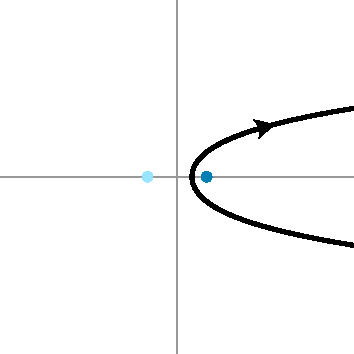
\includegraphics{figures/zeta_contour_3.pdf} \\[1em]
{\small The contour $\gamma_1$ in the $\zeta$ plane.}
\end{center}

It happens\footnote{\textcolor{magenta}{Veronica:} This comes from \cite[equation~15.4.14]{dlmf}.} that for our desired branch of $u$,
\[ \frac{1}{4u^2 - 1} = -F\big(\tfrac{1}{3}, \tfrac{2}{3}; \tfrac{1}{2}; \zeta^2\big), \]
so we can rewrite integral~\ref{integral:mod-bessel-zeta} as
\[ K = \frac{1}{i\sqrt{3}} \int_{\gamma_z} e^{-z\zeta} F\big(\tfrac{1}{3}, \tfrac{2}{3}; \tfrac{1}{2}; \zeta^2\big)\;d\zeta. \]
This gives us an alternate route to the conclusion of Section~\ref{spatial}, which we'll follow below.

In addition to the solutions $g_1$ and $f_0$ from Section~\ref{spatial-success}, equation~\ref{eqn:hypergeom} has the solutions
\begin{alignat*}{2}
g_0 &\;=\;& & F\big(\tfrac{2}{3}, \tfrac{4}{3}; \tfrac{3}{2}; 1-\xi\big) \\
f_1 &\;=\;& (1-\xi)^{-1/2} & F\big(\tfrac{1}{6}, \tfrac{5}{6}; \tfrac{1}{2}; 1-\xi\big),
\end{alignat*}
given by formulas 15.10.13 and 15.10.14 from \cite{dlmf}.

The quadratic transformation identity 15.8.27 from \cite{dlmf} shows \textcolor{magenta}{[verified numerically]} that\footnote{Note that $2\Gamma(\tfrac{1}{2})\Gamma(\tfrac{3}{2}) = 2\Gamma(\tfrac{1}{2})\,\tfrac{1}{2}\Gamma(\tfrac{1}{2}) = \pi$ and $\big[\Gamma(\tfrac{5}{6})\Gamma(\tfrac{7}{6})\big]^{-1} = \big[\Gamma(\tfrac{5}{6})\,\tfrac{1}{6}\Gamma(\tfrac{1}{6})\big]^{-1} = \frac{6\sin(\tfrac{1}{6} \pi)}{\pi} = \frac{3}{\pi}$.}
\[ F\big(\tfrac{1}{3}, \tfrac{2}{3}; \tfrac{1}{2}; \zeta^2\big) = \tfrac{1}{3}(g_1 + g_0), \]
so we have
\[ K = \frac{1}{i\,3\sqrt{3}} \int_{\gamma_z} e^{-z\zeta} (g_1 + g_0)\;d\zeta. \]
The solution $g_1$ is holomorphic on $\zeta \in [1, \infty)$, so it integrates to zero. The solution $g_0$, in contrast, is non-meromorphic at $\zeta = 1$. Along the branch cut $\zeta \in [1, \infty)$, its above-minus-below difference is $-\tfrac{3\sqrt{3}}{2}\,f_0$,
as given\footnote{Note that $\Gamma(\tfrac{3}{2}) \Gamma(\tfrac{1}{2})^{-1} = \tfrac{1}{2}$ and $\big[\Gamma(\tfrac{2}{3})\Gamma(\tfrac{4}{3})\big]^{-1} = \big[\Gamma(\tfrac{2}{3})\,\tfrac{1}{3}\Gamma(\tfrac{1}{3})\big]^{-1} = \frac{3\sin(\tfrac{1}{3} \pi)}{\pi} = \frac{3\sqrt{3}}{2\pi}$.} by equation~15.2.3 from \cite{dlmf}.
Hence,
\begin{align*}
K & = \frac{i}{2} \int^\infty_1 e^{-z\zeta} f_0\;d\zeta \\
e^z K & = \frac{i}{2} \int^\infty_1 e^{-z(\zeta - 1)} f_0\;d\zeta \\
K_1 & = \tfrac{i}{2} \laplace_{\zeta_1} f_0,
\end{align*}
just as we found in Section~\ref{spatial-success}.
\subsection{Another solution}
Section~\ref{contour-argument} associates the solution $K$ of equation~\ref{eqn:mod-bessel} with the solution $g_0$ of equation~\ref{eqn:hypergeom}, which contributes the pole at $\zeta = 1$ of
\[ \frac{du}{d\zeta} = \frac{1}{4u^2 - 1} = \tfrac{1}{3}(g_1 + g_0). \]
The solution $g_1$, which contributes the pole at $\zeta = -1$, is associated with another solution of equation~\ref{eqn:mod-bessel}.

To express this other solution as a Laplace transform, following the method of Section~\ref{spatial-success}, we would use the solution
\[ f_1 = (1-\xi)^{-1/2} F\big(\tfrac{1}{6}, \tfrac{5}{6}; \tfrac{1}{2}; 1-\xi\big) \]
of equation~\ref{eqn:hypergeom}, given by formula~15.10.14 from \cite{dlmf}. This is the only solution, up to scale, which has a fractional power singularity at $\zeta = -1$.

In summary, the contour integration method of solving equation~\ref{eqn:mod-bessel} is associated with the basis
\begin{align*}
g_1 & = F\big(\tfrac{2}{3}, \tfrac{4}{3}; \tfrac{3}{2}; \xi\big) \\
g_0 & = F\big(\tfrac{2}{3}, \tfrac{4}{3}; \tfrac{3}{2}; 1-\xi\big)
\end{align*}
of solutions for equation~\ref{eqn:hypergeom}, given by formulas 15.10.11 and 15.10.13 from \cite{dlmf}. These solutions contribute the poles at $\xi = 1$ and $\xi = 0$, respectively, of a generic solution.

The Laplace transformation method of solving equation~\ref{eqn:mod-bessel}, on the other hand, is associated with the basis
\begin{alignat*}{2}
f_1 &\;=\;& (1-\xi)^{-1/2} & F\big(\tfrac{1}{6}, \tfrac{5}{6}; \tfrac{1}{2}; 1-\xi\big) \\
f_0 &\;=\:& \xi^{-1/2} & F\big(\tfrac{1}{6}, \tfrac{5}{6}; \tfrac{1}{2}; \xi\big)
\end{alignat*}
given by formulas 15.10.14 and 15.10.12 from \cite{dlmf}. These solutions, up to scale, are the only ones with fractional power singularities.

Identities 15.10.18, and 15.10.22 from \cite{dlmf} give the change of basis
\begin{alignat*}{3}
f_1 &\;=\;&\tfrac{1}{\sqrt{3}}\,g_1 &\;+\;& \tfrac{1}{2}\,f_0 \\
f_0 &\;=\;& \tfrac{1}{\sqrt{3}}\,g_0 &\;+\;& \tfrac{1}{2}\,f_1.
\end{alignat*}
Summing these identities, we see that
\[ g_1 + g_0 = \tfrac{\sqrt{3}}{2}\,(f_1 + f_0), \]
giving the alternate decomposition
\[ \frac{du}{d\zeta} = \tfrac{1}{2\sqrt{3}}\,(f_1 + f_0). \]


\subsection{Correspondence with Mari\~{n}o's series}
Let $F_1(z)$ be the holomorphic function corresponding to Mari\~{n}o's formal power series $\varphi_1(z^{-1})$. The formal power series corresponding to $F_1$ will be written in the variable $z$.

\begin{align*}
\Ai(x) & = \tfrac{1}{2\sqrt{\pi}} x^{-1/4} e^{-z} \varphi_1\big(\tfrac{2}{3} z^{-1}\big) \\
& = \tfrac{1}{2\sqrt{\pi}} x^{-1/4} e^{-z} F_1\big(\tfrac{3}{2} z\big) \\
\Ai(x) & = \frac{1}{\pi\sqrt{3}} x^{1/2} K(\tfrac{2}{3} x^{3/2})
\end{align*}
Putting together,
\begin{align*}
\tfrac{1}{2\sqrt{\pi}} x^{-1/4} e^{-z} F_1\big(\tfrac{3}{2} z\big) & = \frac{1}{\pi\sqrt{3}} x^{1/2} K(\tfrac{2}{3} x^{3/2}) \\
\tfrac{\sqrt{3\pi}}{2}\;x^{-3/4} e^{-z} F_1\big(\tfrac{3}{2} z\big) & = K(\tfrac{2}{3} x^{3/2}) \\
\tfrac{\sqrt{3\pi}}{2}\;\big(\tfrac{3}{2} z)^{-1/2} e^{-z} F_1\big(\tfrac{3}{2} z\big) & = K(z) \\
\sqrt{\tfrac{\pi}{2}}\;z^{-1/2} e^{-z} F_1\big(\tfrac{3}{2} z\big) & = K(z) \\
\sqrt{\tfrac{\pi}{2}}\;\big[\laplace^{-1} z^{-1/2}\big] * \big[\laplace^{-1} F_1\big(\tfrac{3}{2} z\big)\big](\zeta - 1) & = k(\zeta) \\
\sqrt{\tfrac{\pi}{2}}\;\left[\Gamma\big({-\tfrac{1}{2}}\big)^{-1} \zeta^{-1/2}\right] * \tfrac{2}{3} f_1\big[\tfrac{2}{3}(\zeta - 1)\big] & = k(\zeta) \\
-\tfrac{1}{3\sqrt{2}}\;\left[\zeta^{-1/2}\right] * f_1\big[\tfrac{2}{3}(\zeta - 1)\big] & = k(\zeta) \\
\end{align*}
Notice that if the hypergeometric differentiation formula holds for fractional derivatives,
\[ \big(\tfrac{\partial}{\partial \xi}\big)^{1/2}F\big(\tfrac{2}{3}, \tfrac{4}{3}; \tfrac{3}{2}; \xi\big) \propto F\big(\tfrac{7}{6}, \tfrac{11}{6}; 2; \xi\big) \]

\subsection{Comparison with other Airy examples}

\subsubsection{Different Borel transform convention} In physics, sometimes it happens that authors find more convenient a different definition of the Borel transform which does not involve the \textit{delta} element for the unit: they define $\mathcal{B}_{\textit{phys}}\colon \C [\![ z^{-1}]\!] \to \C \lbrace \zeta\rbrace$ such that $\mathcal{B}_{\textit{phys}}(z^{-n})\defeq \tfrac{\zeta^n}{n!}$. It is also commun to consider formal power series in small parameters, like $\tilde{\Phi}(\hbar)=\sum_{n\geq 0} a_n\hbar^n$ where $\hbar\to 0$. Then the Borel transform of $\tilde{\Phi}$ is defined as $\tilde{\phi}(\zeta)=\sum_{n\geq 0}a_n\tfrac{\zeta^n}{n!}$. In \cite{Diablerets}, the author studies resurgent properties of the Airy functions: his starting point are the formal solutions of Airy differential equation
\begin{align*}
\tilde{\Phi}_{\mathrm{Ai}}(x)&=\frac{1}{2\sqrt{\pi}}x^{-1/4}e^{-\tfrac{2}{3}x^{3/2}}\tilde{W}_1(x^{-3/2})\\
\tilde{\Phi}_{\mathrm{Bi}}(x)&=\frac{1}{2\sqrt{\pi}}x^{-1/4}e^{\tfrac{2}{3}x^{3/2}}\tilde{W}_2(x^{-3/2})
\end{align*}  
where 
\begin{align*}
\tilde{W}_{1,2}(\hbar)=\sum_{n=0}^{\infty}\frac{1}{2\pi}\left(\mp\frac{3}{4}\right)^{n}\frac{\Gamma(n+\frac{5}{6})\Gamma(n+\frac{1}{6})}{n!}\hbar^n
\end{align*}
Notice that $\tilde{W}_{1,2}(\hbar)$ are proportional to $\tilde{W}_{\pm}(z)$ with $z=\hbar^{-1}$. However, their Borel transforms are two different hypergeometric functions:
\begin{align*}
w_{1,2}(\zeta)&\defeq\mathcal{B}_{\textit{phys}}(\tilde{W}_{1,2})(\zeta)\\
&=\sum_{n=0}^{\infty}\frac{1}{2\pi}\left(\mp\frac{3}{4}\right)^{n}\frac{\Gamma(n+\frac{5}{6})\Gamma(n+\frac{1}{6})}{n!}\frac{\zeta^n}{n!}\\
&={}_2F_1\left(\frac{1}{6},\frac{5}{6};1;\mp\frac{3}{4}\zeta\right) \\
\mathcal{B}(\tilde{W}_{1,2})(\zeta)&=\frac{1}{2\pi}\delta+\sum_{n=1}^{\infty} \frac{1}{2\pi}\left(\mp\frac{3}{4}\right)^{n}\frac{\Gamma(n+\frac{5}{6})\Gamma(n+\frac{1}{6})}{n!}\frac{\zeta^{n-1}}{(n-1)!}\\
&=\frac{1}{2\pi}\delta+\sum_{n=0}^{\infty} \frac{1}{2\pi}\left(\mp\frac{3}{4}\right)^{n+1}\frac{\Gamma(n+1+\frac{5}{6})\Gamma(n+1+\frac{1}{6})}{(n+1)!}\frac{\zeta^{n}}{n!}\\
&=\frac{1}{2\pi}\delta\mp\frac{3}{4}\sum_{n=0}^{\infty} \frac{1}{2\pi}\left(\mp\frac{3}{4}\right)^{n}\frac{\Gamma(n+\frac{11}{6})\Gamma(n+\frac{7}{6})}{\Gamma(n+2)}\frac{\zeta^{n}}{n!}\\
&=\frac{1}{2\pi}\delta\mp\frac{5}{48} {}_2F_1\left(\frac{7}{6},\frac{11}{6};2;\mp\frac{3}{4}\zeta\right)%\\
%&=\frac{1}{2\pi}\delta\mp \frac{5}{48}\frac{1}{c_{1,2}}w_{\pm}(\zeta)
%w_{\pm}(\zeta)&=c_{1,2}\,\,{}_2F_1\left(\frac{7}{6},\frac{11}{6};2;\mp\frac{3}{4}\zeta\right) &\qquad \text{see \eqref{eq:hat+}\eqref{eq:hat-}}
\end{align*}
%That ambiguity comes from the different definitions of Borel transforms: 
%\begin{align*}
%\mathcal{B}(\tilde{W}_{1,2})(\zeta)&=\frac{1}{2\pi}\delta+\sum_{n=1}^{\infty} \frac{1}{2\pi}\left(\mp\frac{3}{4}\right)^{n}\frac{\Gamma(n+\frac{5}{6})\Gamma(n+\frac{1}{6})}{n!}\frac{\zeta^{n-1}}{(n-1)!}\\
%&=\frac{1}{2\pi}\delta+\sum_{n=0}^{\infty} \frac{1}{2\pi}\left(\mp\frac{3}{4}\right)^{n+1}\frac{\Gamma(n+1+\frac{5}{6})\Gamma(n+1+\frac{1}{6})}{(n+1)!}\frac{\zeta^{n}}{n!}\\
%&=\frac{1}{2\pi}\delta\mp\frac{3}{4}\sum_{n=0}^{\infty} \frac{1}{2\pi}\left(\mp\frac{3}{4}\right)^{n}\frac{\Gamma(n+\frac{11}{6})\Gamma(n+\frac{7}{6})}{\Gamma(n+2)}\frac{\zeta^{n}}{n!}\\
%&=\frac{1}{2\pi}\delta\mp\frac{5}{48} {}_2F_1\left(\frac{7}{6},\frac{11}{6};2;\mp\frac{3}{4}\zeta\right)%\\
%%&=\frac{1}{2\pi}\delta\mp \frac{5}{48}\frac{1}{c_{1,2}}w_{\pm}(\zeta)
%\end{align*}  

Comparing $\mathcal{B}(\tilde{W}_{1,2})(\zeta)$ with $\hat{w}_{\pm}$ in \eqref{hat+}\eqref{hat-}, they differ only by a constant which multiplies the $\delta$.
\subsubsection{Integral formula for hypergeometric functions}

In \cite{MS16} the author studies summability and resurgent properties of solutions of the Airy equation. He defines the formal series $\tilde{\Phi}_{\pm}(z)\defeq \sum_{n=0}^{\infty}\frac{1}{2\pi}\left(\mp\frac{1}{2}\right)^{n}\frac{\Gamma(n+\frac{5}{6})\Gamma(n+\frac{1}{6})}{n!}z^{-n}$ such that 

\begin{align*}
\Phi_{\mathrm{Ai}}(y)&=\frac{1}{2\sqrt{\pi}}y^{-1/4}e^{-\tfrac{2}{3}y^{3/2}}\mathcal{L}\circ\mathcal{B}\tilde{\Phi}_{+}\left(\tfrac{2}{3}y^{3/2}\right)\\
\Phi_{\mathrm{Bi}}(y)&=\frac{1}{2\sqrt{\pi}}y^{-1/4}e^{\tfrac{2}{3}y^{3/2}}\mathcal{L}\circ\mathcal{B}\tilde{\Phi}_{-}\left(\tfrac{2}{3}y^{3/2}\right)
\end{align*}

Notice that $\tilde{W}_{1,2}(\tfrac{2}{3}\hbar)=\tilde{\Phi}_{\pm}(z)$ for $\hbar=z^{-1}$, hence 

\begin{align*}
\tilde{\phi}_{+}(\zeta)&=\mathcal{B}\tilde{W}_{1}(\tfrac{2}{3}\zeta)=\frac{1}{2\pi}\delta-\frac{5}{48} {}_2F_1\left(\frac{7}{6},\frac{11}{6};2;-\frac{\zeta}{2}\right) \\
\tilde{\phi}_{-}(\zeta)&=\mathcal{B}\tilde{W}_{2}(\tfrac{2}{3}\zeta)=\frac{1}{2\pi}\delta+\frac{5}{48} {}_2F_1\left(\frac{7}{6},\frac{11}{6};2;\frac{\zeta}{2}\right) 
\end{align*}
which up to a constant factor for $\delta$, they agree with our results. 

However, the author adopts a different approach to compute $\tilde{\phi}_{\pm}(\zeta)$: he argues that $\Phi_{\mathrm{Ai}}, \Phi_{\mathrm{Bi}}$ are solutions of Airy equation if and only if 

\begin{align*}
\tilde{\phi}_+(\zeta)=\delta+\frac{d}{d\zeta}\tilde{\chi}(\zeta)  \qquad \tilde{\phi}_-(\zeta)=\delta-\frac{d}{d\zeta}\tilde{\chi}(-\zeta)
\end{align*}
 where $\chi(\zeta)=\frac{2^{1/6}}{\Gamma(1/6)\Gamma(5/6)}(2\zeta+\zeta^2)^{-1/6}\ast \zeta^{-5/6}$. Function $\chi(\zeta)$ is an hypergeometric function:

\begin{align*}
\chi(\zeta)&=\frac{2^{1/6}}{\Gamma(1/6)\Gamma(5/6)}(2\zeta+\zeta^2)^{-1/6}\ast \zeta^{-5/6}\\
&=\frac{2^{1/6}}{\Gamma(1/6)\Gamma(5/6)}\int_0^{\zeta}(2\zeta'+\zeta'^2)^{-1/6} (\zeta-\zeta')^{-5/6}d\zeta'\\
&=\frac{2^{1/6}}{\Gamma(1/6)\Gamma(5/6)}\int_0^{1}(\zeta t)^{-1/6}(2+\zeta t)^{-1/6} (\zeta-\zeta t)^{-5/6} \zeta dt\\
&=\frac{2^{1/6}}{\Gamma(1/6)\Gamma(5/6)}\int_0^{1} t^{-1/6} 2^{-1/6}(1+\zeta t)^{-1/6} (1-t)^{-5/6}d\zeta'\\
&=\frac{1}{\Gamma(1/6)\Gamma(5/6)}\int_0^{1} t^{-1/6} (1+\zeta t)^{-1/6} (1-t)^{-5/6}d\zeta'\\
&={}_2F_1\left(\frac{1}{6},\frac{5}{6};1;-\frac{\zeta}{2}\right)
\end{align*}
where in the last step we use the Euler formula for hypergeometric functions (see \eqref{Euler formula}). Finally, we take the derivative 

\begin{align*}
\tilde{\phi}_+(\zeta)&=\delta-\frac{1}{2}\frac{5}{36}\,\, {}_2F_1\left(\frac{7}{6},\frac{11}{6};2;-\frac{\zeta}{2}\right)=\delta-\frac{2}{3}\frac{5}{48} {}_2F_1\left(\frac{7}{6},\frac{11}{6};2;-\frac{\zeta}{2}\right)\\
\tilde{\phi}_-(\zeta)&=\delta+\frac{1}{2}\frac{5}{36}\,\, {}_2F_1\left(\frac{7}{6},\frac{11}{6};2;\frac{\zeta}{2}\right)=\delta+\frac{2}{3}\frac{5}{48} {}_2F_1\left(\frac{7}{6},\frac{11}{6};2;\frac{\zeta}{2}\right).
\end{align*} 

The main advantage of writing Gauss hypergeometric functions as a convolution product relies on Ecalle's singularity theory. Indeed $(2\zeta+\zeta^2)^{-1/6}$ extends analytically to the universal cover of $\C\setminus\lbrace 0,-2\rbrace$ and the convolution with $\zeta^{-5/6}$ does not change the set of singularities (see \textbf{Sauzin notes}). Therefore, from the expression of $\chi(\zeta)$ as a convolution product, the resurgent properties of $\tilde{\phi}_{\pm}(\zeta)$ are evident.  

\subsubsection{Comparison with exact WKB}

Kawai and Takei study the WKB analysis of the equation

\begin{equation}
\label{WKB_Airy} 
\left[\left(\frac{d}{dx}\right)^2 - \eta^2 x \right] \psi(x, \eta) = 0 
\end{equation}
as $\eta\to\infty$. They define $\psi_B(x, y)$ as the inverse Laplace transform of $\psi(x, \eta)$ with respect to $\eta$. In the coordinates $t=yx^{-3/2}$ they find an explicit formula for $\psi_B(x,y)$ in terms of Gauss hypergeometric functions:
\begin{align*}
\psi_{+,B}(x,y)&=\frac{1}{x}\phi_+(t)=\frac{\sqrt{3}}{2\sqrt{\pi}}\frac{1}{x}s^{-1/2}\, {}_2F_1\left(\frac{1}{6},\frac{5}{6};\frac{1}{2};s\right)\\
\psi_{-,B}(x,y)&=\frac{1}{x}\phi_-(t)=\frac{\sqrt{3}}{2\sqrt{\pi}}\frac{1}{x}(1-s)^{-1/2}\, {}_2F_1\left(\frac{1}{6},\frac{5}{6};\frac{1}{2};1-s\right)
\end{align*}
where $s=3t/4+1/2$. 
The same hypergeometric functions have been computed in Section ?? as the Borel transform of the formal solutions of the Airy equation

\begin{equation}
\label{Airy}
\left[\left(\frac{d}{dw}\right)^2 -  w \right] f(w) = 0.
\end{equation}

Although the two equations look closely related (they are equivalent by the change of coordinates $w=x\eta^{2/3}$), the Borel transform of $\psi$ is computed with respect to $\eta x^{3/2}$ (which is the conjugate variable of $t$) while the Borel transform of $f(w)$ is computed with respect to $w$. So we need to find a different change of coordinates to explain why the Borel transforms of $\psi(x,\eta)$ and $f(w)$ are given by the same hypergeometric function. 

First of all notice that if $\eta$ and $y$ are conjugate variables under Borel transform, meaning 
\begin{align*}
\sum_{n\geq 0}a_n\eta^{-n-1}  \overset{\mathcal{B}}{\longrightarrow} \sum_{n\geq 0}\frac{a_n}{n!} y^{n} 
\end{align*} 
then $t=yx^{-3/2}$ is the conjugate variable of $q=\eta x^{3/2}$ up to correction by a factor of $x^{-3/2}$
\begin{align*}
\sum_{n\geq 0}a_nq^{-n-1}=\sum_{n\geq 0}a_nx^{-3/2(n+1)}\eta^{-n-1}  \overset{\mathcal{B}}{\longrightarrow} \sum_{n\geq 0}\frac{a_nx^{-3/2(n+1)}}{n!} y^{n}=x^{-3/2}\sum_{n\geq 0}\frac{a_n}{n!} t^{n}. 
\end{align*}
In addition, $\psi_{B,\pm}(x,y)=\frac{1}{x}\phi_{\pm}(t)$, therefore we expect that $\psi(x,\eta)=x^{1/2}\Phi(q)$. Assume that $\psi(x,y)$ is a solution of \eqref{WKB_Airy}, then $\Phi(q)$ solves 
\begin{equation}
\label{eq_Phi}
\left[\left(\frac{d}{dx}\right)^2+x^{-1}\frac{d}{dx}-\frac{1}{4}x^{-2} - \eta^2 x \right] \Phi(q) = 0
\end{equation}

\begin{proof}
\begin{align*}
&\left[\left(\frac{d}{dx}\right)^2 - \eta^2 x \right] \psi(x, \eta) = 0\\
&\left[\left(\frac{d}{dx}\right)^2 - \eta^2 x \right] x^{1/2}\Phi(q) = 0\\
&\frac{d}{dx}\left[\frac{1}{2}x^{-1/2}\Phi+x^{1/2}\frac{d}{dx}\Phi\right]-\eta^2x^{3/2}\Phi=0\\
&-\frac{1}{4}x^{-3/2}\Phi+\frac{1}{2}x^{-1/2}\frac{d}{dx}\Phi+\frac{1}{2}x^{-1/2}\frac{d}{dx}\Phi+x^{1/2}\left(\frac{d}{dx}\right)^2\Phi-\eta^2x^{3/2}\Phi=0\\
&\left[x^{1/2}\left(\frac{d}{dx}\right)^2+x^{-1/2}\frac{d}{dx}-\frac{1}{4}x^{-3/2}-\eta^2x^{3/2}\right]\Phi=0\\
&\left[\left(\frac{d}{dx}\right)^2+x^{-1}\frac{d}{dx}-\frac{1}{4}x^{-2}-\eta^2x\right]\Phi=0
\end{align*}
\end{proof}
Now rewrite \eqref{eq_Phi} in the coordinates $q=\eta x^{3/2}$: 
\begin{align*}
&\left[\left(\frac{d}{dx}\right)^2+x^{-1}\frac{d}{dx}-\frac{1}{4}x^{-2}-\eta^2x\right]\Phi=0\\
&\left[\frac{9}{4}\eta^2x\left(\frac{d}{dq}\right)^2+\frac{3}{4}\eta x^{-1/2}\frac{d}{dq}+x^{-1}\cdot\frac{3}{2}\, \eta\,  x^{1/2}\frac{d}{dq}-\frac{1}{4}x^{-2}-\eta^2x\right]\Phi=0\\
&\left[\eta^2x\left(\frac{d}{dq}\right)^2+\frac{1}{3}\eta x^{-1/2}\frac{d}{dq}+\frac{2}{3}\, \eta\,  x^{-1/2}\frac{d}{dq}-\frac{1}{9}x^{-2}-\frac{4}{9}\eta^2x\right]\Phi=0\\
&\left[\eta^2\left(\frac{d}{dq}\right)^2+\eta x^{-3/2}\frac{d}{dq}-\frac{1}{9}x^{-3}-\frac{4}{9}\eta^2\right]\Phi=0\\
&\left[\left(\frac{d}{dq}\right)^2+\eta^{-1} x^{-3/2}\frac{d}{dq}-\frac{1}{9}\eta^{-2}x^{-3}-\frac{4}{9}\right]\Phi=0\\
&\left[\left(\frac{d}{dq}\right)^2+q^{-1}\frac{d}{dq}-\frac{1}{9}q^{-2}-\frac{4}{9}\right]\Phi=0
\end{align*}

therefore $\Phi(q)$ is a solution of the transform Airy equation (see draft2).  

\bibliographystyle{plain}
\bibliography{airy-resurgence}

\end{document}